% Options for packages loaded elsewhere
\PassOptionsToPackage{unicode}{hyperref}
\PassOptionsToPackage{hyphens}{url}
%
\documentclass[
  8pt,
  ignorenonframetext,
]{beamer}
\usepackage{pgfpages}
\setbeamertemplate{caption}[numbered]
\setbeamertemplate{caption label separator}{: }
\setbeamercolor{caption name}{fg=normal text.fg}
\beamertemplatenavigationsymbolsempty
% Prevent slide breaks in the middle of a paragraph
\widowpenalties 1 10000
\raggedbottom
\setbeamertemplate{part page}{
  \centering
  \begin{beamercolorbox}[sep=16pt,center]{part title}
    \usebeamerfont{part title}\insertpart\par
  \end{beamercolorbox}
}
\setbeamertemplate{section page}{
  \centering
  \begin{beamercolorbox}[sep=12pt,center]{part title}
    \usebeamerfont{section title}\insertsection\par
  \end{beamercolorbox}
}
\setbeamertemplate{subsection page}{
  \centering
  \begin{beamercolorbox}[sep=8pt,center]{part title}
    \usebeamerfont{subsection title}\insertsubsection\par
  \end{beamercolorbox}
}
\AtBeginPart{
  \frame{\partpage}
}
\AtBeginSection{
  \ifbibliography
  \else
    \frame{\sectionpage}
  \fi
}
\AtBeginSubsection{
  \frame{\subsectionpage}
}
\usepackage{amsmath,amssymb}
\usepackage{lmodern}
\usepackage{iftex}
\ifPDFTeX
  \usepackage[T1]{fontenc}
  \usepackage[utf8]{inputenc}
  \usepackage{textcomp} % provide euro and other symbols
\else % if luatex or xetex
  \usepackage{unicode-math}
  \defaultfontfeatures{Scale=MatchLowercase}
  \defaultfontfeatures[\rmfamily]{Ligatures=TeX,Scale=1}
\fi
% Use upquote if available, for straight quotes in verbatim environments
\IfFileExists{upquote.sty}{\usepackage{upquote}}{}
\IfFileExists{microtype.sty}{% use microtype if available
  \usepackage[]{microtype}
  \UseMicrotypeSet[protrusion]{basicmath} % disable protrusion for tt fonts
}{}
\makeatletter
\@ifundefined{KOMAClassName}{% if non-KOMA class
  \IfFileExists{parskip.sty}{%
    \usepackage{parskip}
  }{% else
    \setlength{\parindent}{0pt}
    \setlength{\parskip}{6pt plus 2pt minus 1pt}}
}{% if KOMA class
  \KOMAoptions{parskip=half}}
\makeatother
\usepackage{xcolor}
\newif\ifbibliography
\usepackage{longtable,booktabs,array}
\usepackage{calc} % for calculating minipage widths
\usepackage{caption}
% Make caption package work with longtable
\makeatletter
\def\fnum@table{\tablename~\thetable}
\makeatother
\setlength{\emergencystretch}{3em} % prevent overfull lines
\providecommand{\tightlist}{%
  \setlength{\itemsep}{0pt}\setlength{\parskip}{0pt}}
\setcounter{secnumdepth}{-\maxdimen} % remove section numbering
\newlength{\cslhangindent}
\setlength{\cslhangindent}{1.5em}
\newlength{\csllabelwidth}
\setlength{\csllabelwidth}{3em}
\newlength{\cslentryspacingunit} % times entry-spacing
\setlength{\cslentryspacingunit}{\parskip}
\newenvironment{CSLReferences}[2] % #1 hanging-ident, #2 entry spacing
 {% don't indent paragraphs
  \setlength{\parindent}{0pt}
  % turn on hanging indent if param 1 is 1
  \ifodd #1
  \let\oldpar\par
  \def\par{\hangindent=\cslhangindent\oldpar}
  \fi
  % set entry spacing
  \setlength{\parskip}{#2\cslentryspacingunit}
 }%
 {}
\usepackage{calc}
\newcommand{\CSLBlock}[1]{#1\hfill\break}
\newcommand{\CSLLeftMargin}[1]{\parbox[t]{\csllabelwidth}{#1}}
\newcommand{\CSLRightInline}[1]{\parbox[t]{\linewidth - \csllabelwidth}{#1}\break}
\newcommand{\CSLIndent}[1]{\hspace{\cslhangindent}#1}
% type setting
% ------------------------------------------------------------------------------
\usepackage[german]{babel}     

% fonts
% ------------------------------------------------------------------------------
\usefonttheme{professionalfonts}

% slide title and horizontal line
% ------------------------------------------------------------------------------
\setbeamertemplate{frametitle}{%
    \vskip-30pt \color{black}\large%
    \begin{minipage}[b][23pt]{120mm}%
    \flushleft\insertframetitle%
    \end{minipage}%
}

\setbeamertemplate{headline}										
{
\vskip10pt\hfill\hspace{3.5mm} 										 
\vskip15pt\color{black}\rule{\textwidth}{0.4pt} 					 
}

% slide number
% ---------------------------------------------------------------
\setbeamertemplate{navigation symbols}{}
\setbeamertemplate{footline}
{
\vskip5pt
\vskip2pt
\makebox[123mm]{\hspace{7.5mm}
\hfill Psychologische Forschungsmethoden $\vert$ 
\copyright $ $ 2023 Dirk Ostwald CC BY-SA 4.0 $\vert$ 
Folie \insertframenumber}
\vskip4pt
}

% block color scheme
% ------------------------------------------------------------------------------
% colors
\definecolor{white}{RGB}{255,255,255}
\definecolor{grey}{RGB}{235,235,235}
\definecolor{lightgrey}{RGB}{245,245,245}
\definecolor{LightBlue}{RGB}{220,220,255}
\definecolor{darkblue}{RGB}{51, 51, 153}

% definitions and theorems
\setbeamercolor{block title}{fg = black, bg = grey}
\setbeamercolor{block body}{fg = black, bg = lightgrey}

% general line spacing 
% ------------------------------------------------------------------------------
\linespread{1.3}

% local line spacing
% ------------------------------------------------------------------------------
\usepackage{setspace}

% colors
% -----------------------------------------------------------------------------
\usepackage{color}

% justified text
% ------------------------------------------------------------------------------
\usepackage{ragged2e}
\usepackage{etoolbox}
\apptocmd{\frame}{}{\justifying}{}

% bullet point lists
% -----------------------------------------------------------------------------
\setbeamertemplate{itemize item}[circle]
\setbeamertemplate{itemize subitem}[circle]
\setbeamertemplate{itemize subsubitem}[circle]
\setbeamercolor{itemize item}{fg = black}
\setbeamercolor{itemize subitem}{fg = black}
\setbeamercolor{itemize subsubitem}{fg = black}
\setbeamercolor{enumerate item}{fg = black}
\setbeamercolor{enumerate subitem}{fg = black}
\setbeamercolor{enumerate subsubitem}{fg = black}
\setbeamerfont{itemize/enumerate body}{}
\setbeamerfont{itemize/enumerate subbody}{size = \normalsize}
\setbeamerfont{itemize/enumerate subsubbody}{size = \normalsize}

% color links
% ------------------------------------------------------------------------------
\usepackage{hyperref}
\definecolor{urls}{RGB}{204,0,0}
\hypersetup{colorlinks, citecolor = darkblue, urlcolor = urls}


% additional math commands
% ------------------------------------------------------------------------------
\usepackage{bm}                                         % bold math symbols
\newcommand{\niton}{\not\owns}

% text highlighting
% ------------------------------------------------------------------------------
\usepackage{soul}
\makeatletter
\let\HL\hl
\renewcommand\hl{%
  \let\set@color\beamerorig@set@color
  \let\reset@color\beamerorig@reset@color
  \HL}
\makeatother

% equation highlighting
% -----------------------------------------------------------------------------
\newcommand{\highlight}[2][yellow]{\mathchoice%
  {\colorbox{#1}{$\displaystyle#2$}}%
  {\colorbox{#1}{$\textstyle#2$}}%
  {\colorbox{#1}{$\scriptstyle#2$}}%
  {\colorbox{#1}{$\scriptscriptstyle#2$}}}%

% additional mathematical operators
% ------------------------------------------------------------------------------
\DeclareMathOperator*{\argmax}{arg\,max}
\DeclareMathOperator*{\argmin}{arg\,min}

\ifLuaTeX
  \usepackage{selnolig}  % disable illegal ligatures
\fi
\IfFileExists{bookmark.sty}{\usepackage{bookmark}}{\usepackage{hyperref}}
\IfFileExists{xurl.sty}{\usepackage{xurl}}{} % add URL line breaks if available
\urlstyle{same} % disable monospaced font for URLs
\hypersetup{
  hidelinks,
  pdfcreator={LaTeX via pandoc}}

\author{}
\date{\vspace{-2.5em}}

\begin{document}

\begin{frame}[plain]{}
\protect\hypertarget{section}{}
\center

\begin{center}
\includegraphics[width=0.2\linewidth]{3_Abbildungen/pfm_3_otto} \end{center}

\vspace{2mm}

\Large

Psychologische Forschungsmethoden \vspace{6mm}

\normalsize

BSc Philosophie-Neurowissenschaften-Kognition WiSe 2022/23

BSc Psychologie WiSe 2022/23

\large
\vspace{6mm}

Prof.~Dr.~Dirk Ostwald
\end{frame}

\begin{frame}[plain]{}
\protect\hypertarget{section-1}{}
\vfill
\center
\huge

\textcolor{black}{(3) Psychologische Daten} \vfill
\end{frame}

\begin{frame}{}
\protect\hypertarget{section-2}{}
\Large
\setstretch{3}
\vfill

Überblick

Verhaltensdaten

Physiologische Daten

Selbstkontrollfragen \vfill
\end{frame}

\begin{frame}{Überblick}
\protect\hypertarget{uxfcberblick}{}
\begin{center}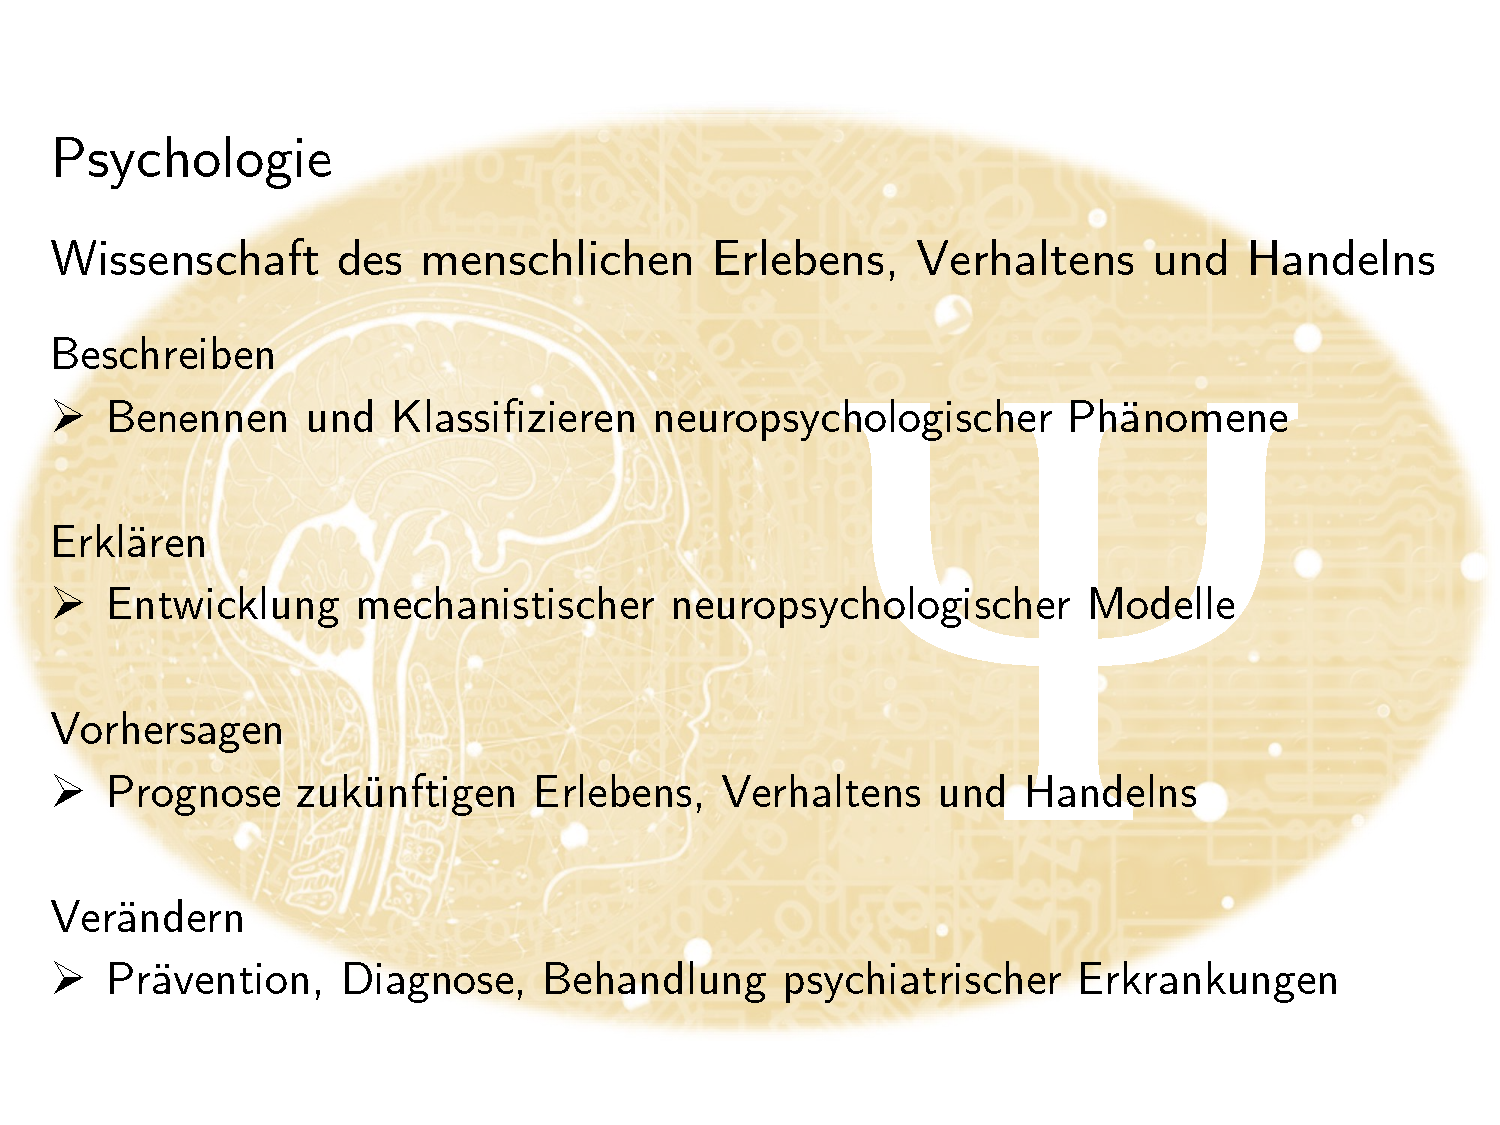
\includegraphics[width=1\linewidth]{3_Abbildungen/pfm_3_psychologie} \end{center}
\end{frame}

\begin{frame}{Überblick}
\protect\hypertarget{uxfcberblick-1}{}
\begin{center}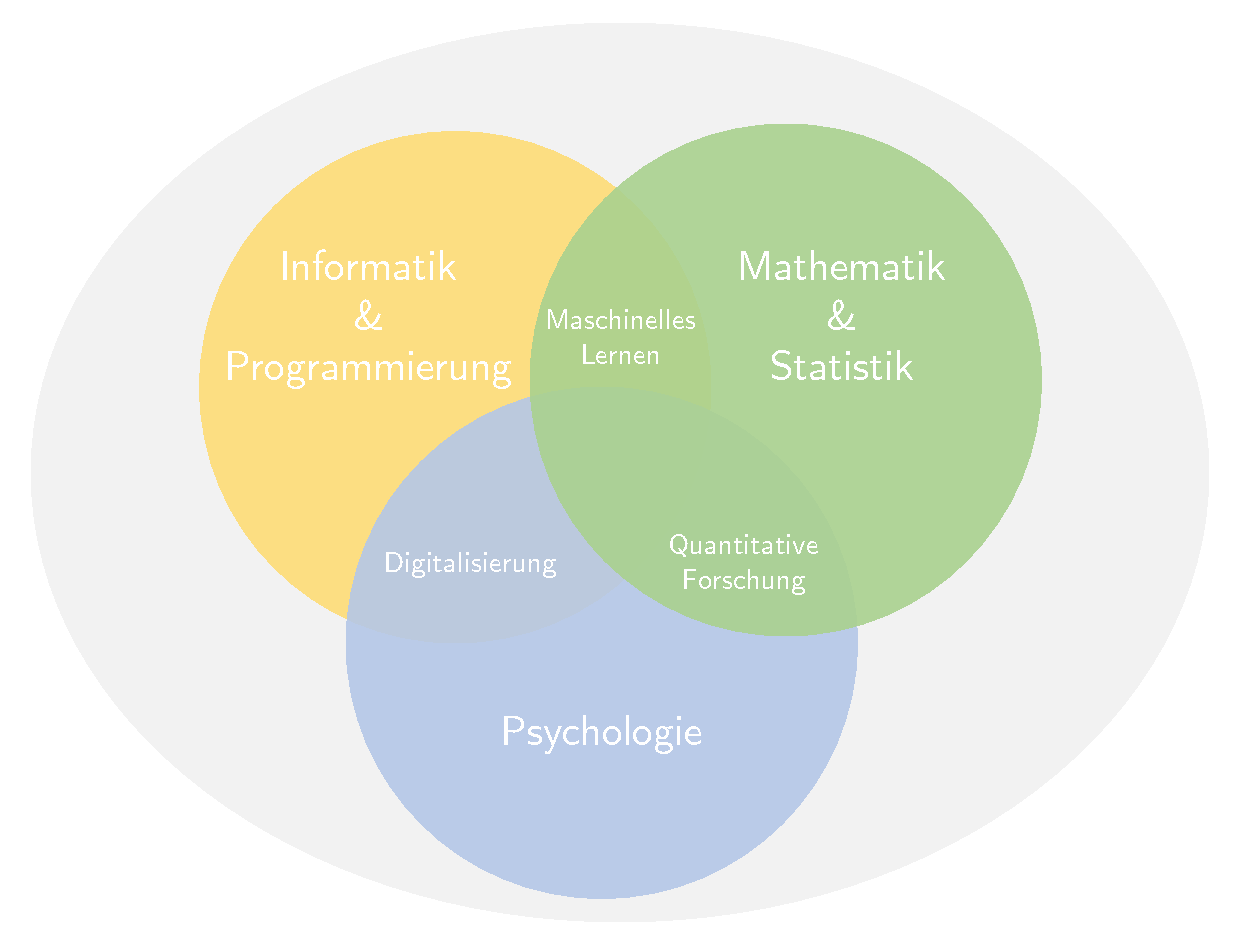
\includegraphics[width=0.9\linewidth]{3_Abbildungen/pfm_3_moderne_psychologie} \end{center}
\end{frame}

\begin{frame}{Überblick}
\protect\hypertarget{uxfcberblick-2}{}
\begin{center}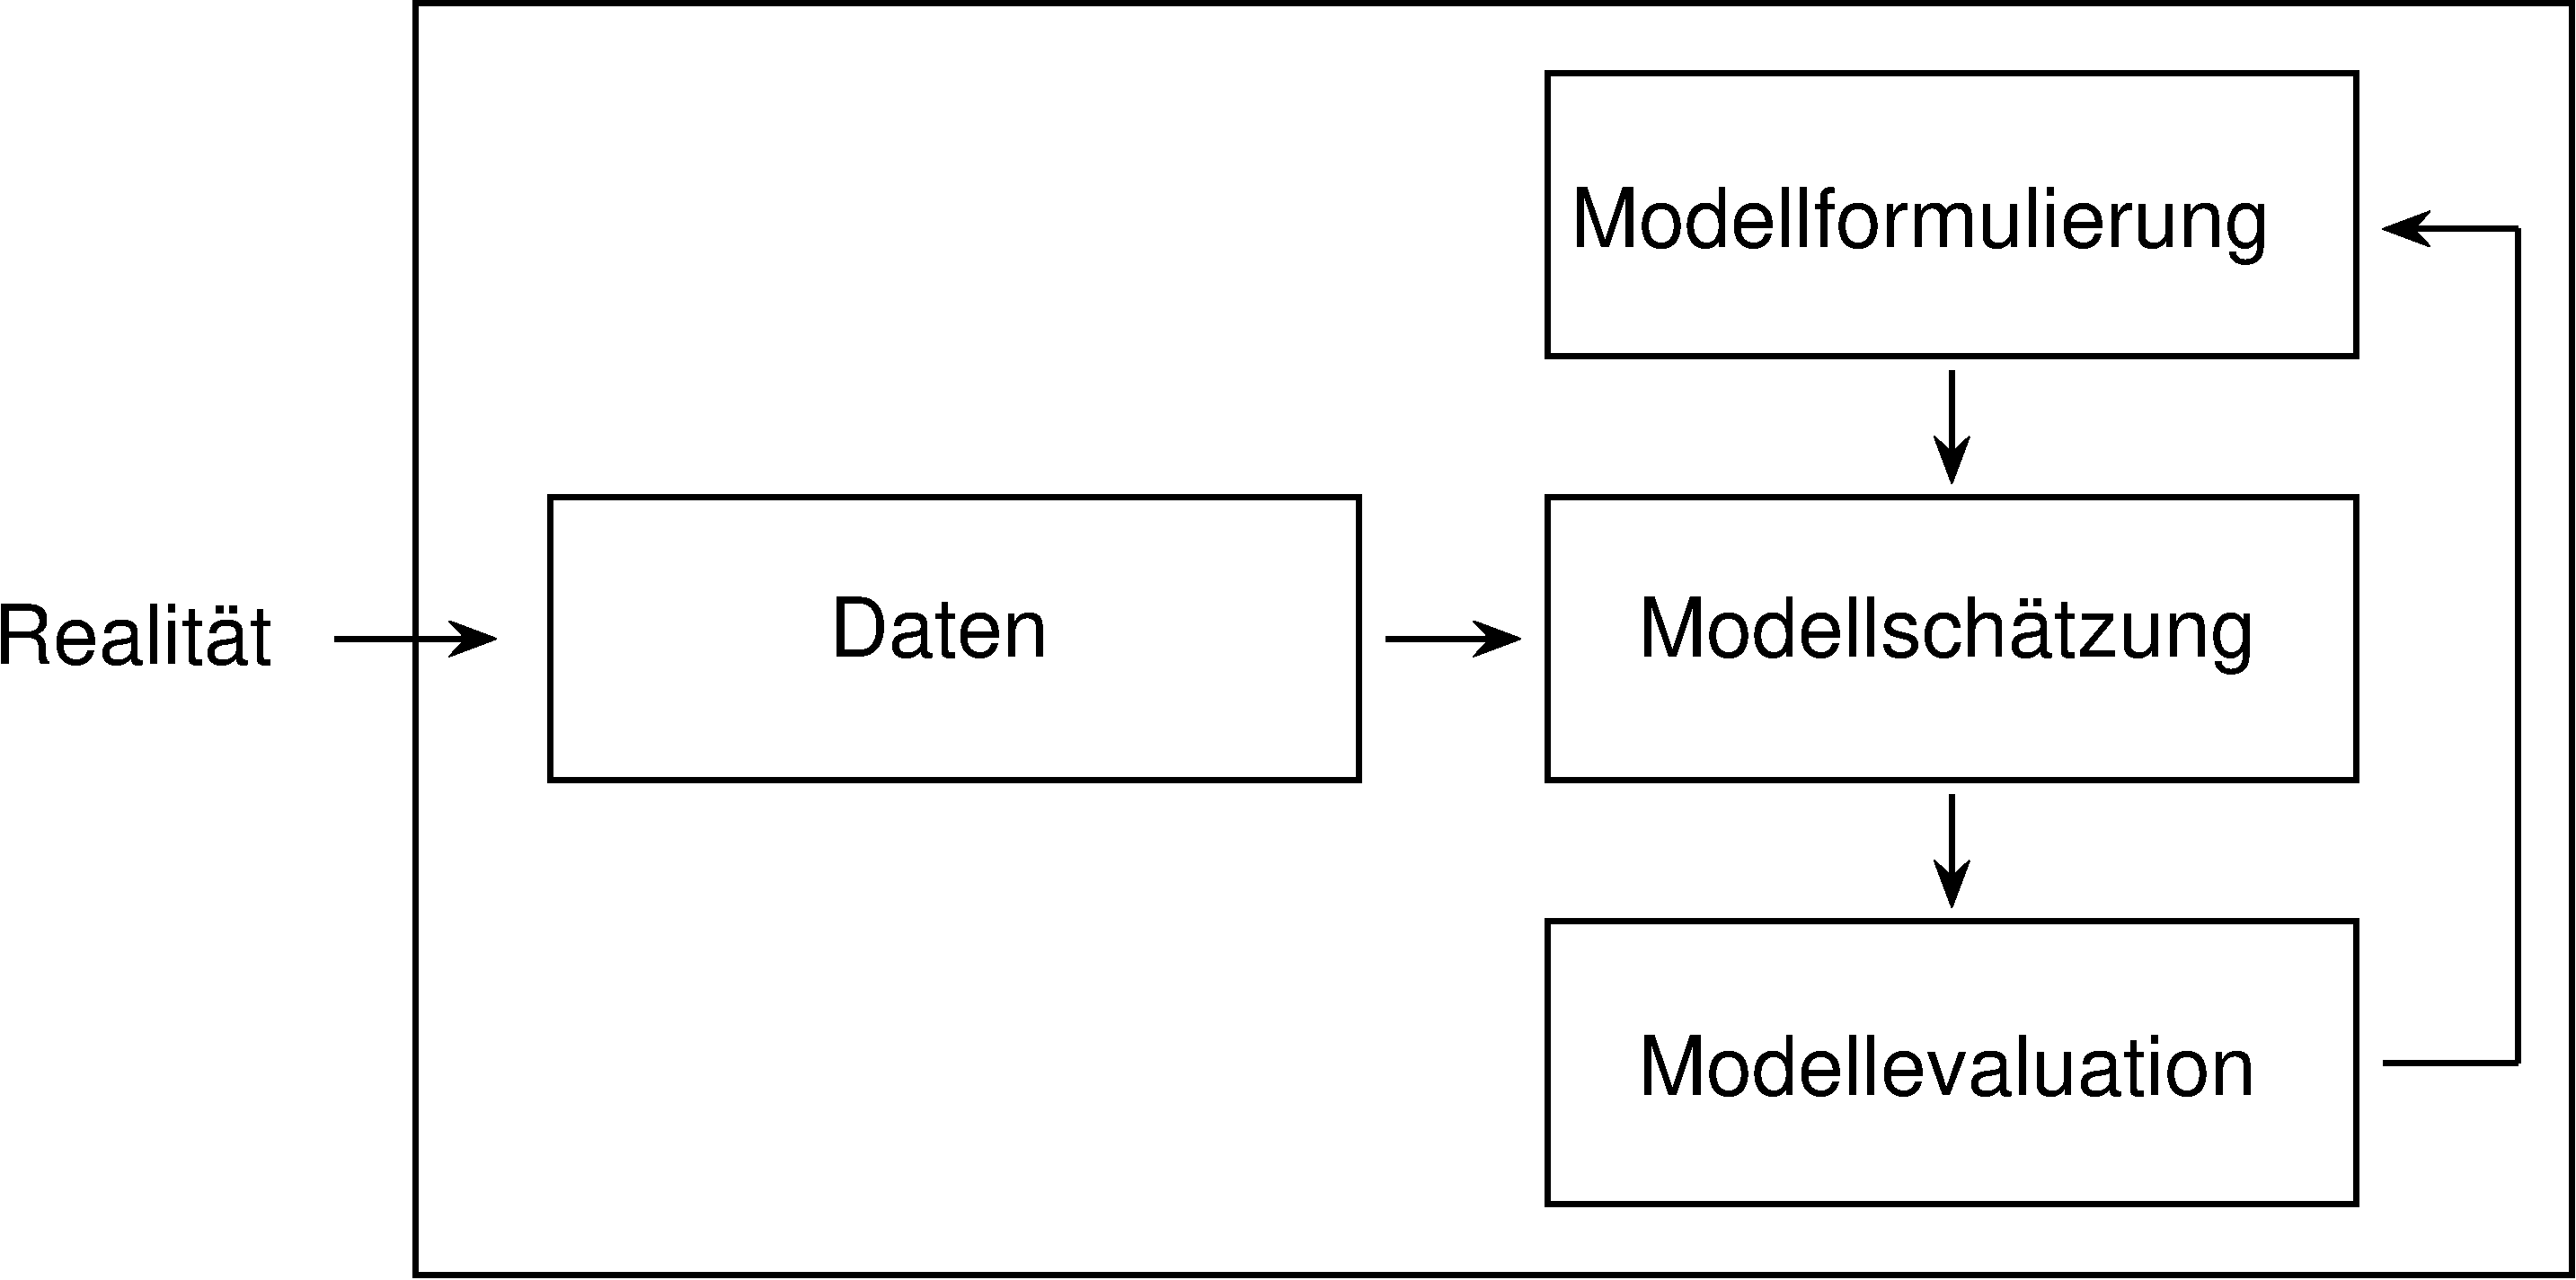
\includegraphics[width=1\linewidth]{3_Abbildungen/pfm_3_modellbasierte_datenwissenschaft} \end{center}
\end{frame}

\begin{frame}{Überblick}
\protect\hypertarget{uxfcberblick-3}{}
\textcolor{darkblue}{Psychologische Daten}

\small

Der Umgang mit Forschungsdaten im Fach Psychologie (DPGS Stellungnahme
2017)

\footnotesize

\emph{Felix Schönbrodt, Mario Gollwitzer und Andrea Abele-Brehm (2017)
Psychologische Rundschau}

\justifying (\ldots) Rohdaten sind die Ursprungsaufzeichnungen, z.B.
Kreuze auf einem Papierfragebogen, Zeichnungen oder auch Audio- oder
Videoaufnahmen. Mit Primärdaten ist die erste Übertragung der Rohdaten
in ein digitales Format gemeint, also z.B. Code „1`` für eine Ja-Antwort
usw.

Somit sind Primärdaten in der Psychologie vollkommen unbearbeitete
(\ldots) quantitative und qualitative Daten, zum Beispiel

\begin{itemize}
\tightlist
\item
  \justifying bei Experimenten alle manipulierten und gemessenen
  Variablen für jeden Experimentaldurchgang jeder Person;
\item
  bei Fragebögen die Antworten jeder Person auf jedem Item;
\item
  bei Freitext-Eingaben der Originalwortlaut (\ldots);
\item
  digitalisierte Videoaufnahmen (\ldots);
\item
  Downloads oder Screenshots von Inhalten sozialer Medien (\ldots);
\item
  bei (neuro)physiologischen Daten (wie EEG- oder fMRT-Daten)
  verlustfrei umgewandelte Daten in einem standardisierten
  Rohdatenformat (\ldots), die nicht aggregiert sind und nicht nur auf
  wenige „regions of interest`` beschränkt sind.
\end{itemize}

\flushright

Schönbrodt, Gollwitzer, and Abele-Brehm (2017)
\end{frame}

\begin{frame}{Überblick}
\protect\hypertarget{uxfcberblick-4}{}
\textcolor{darkblue}{Das deutsche psychologische Dateninstitut}

\small

Leibniz-Institut für Psychologie in Trier der
\href{https://www.leibniz-gemeinschaft.de/}{\textcolor{blue}{Leibniz Gemeinschaft}}

\begin{itemize}
\tightlist
\item
  Bis 2020: Leibniz-Zentrum für Psychologische Information und
  Dokumentation (ZPID)
\end{itemize}

\begin{center}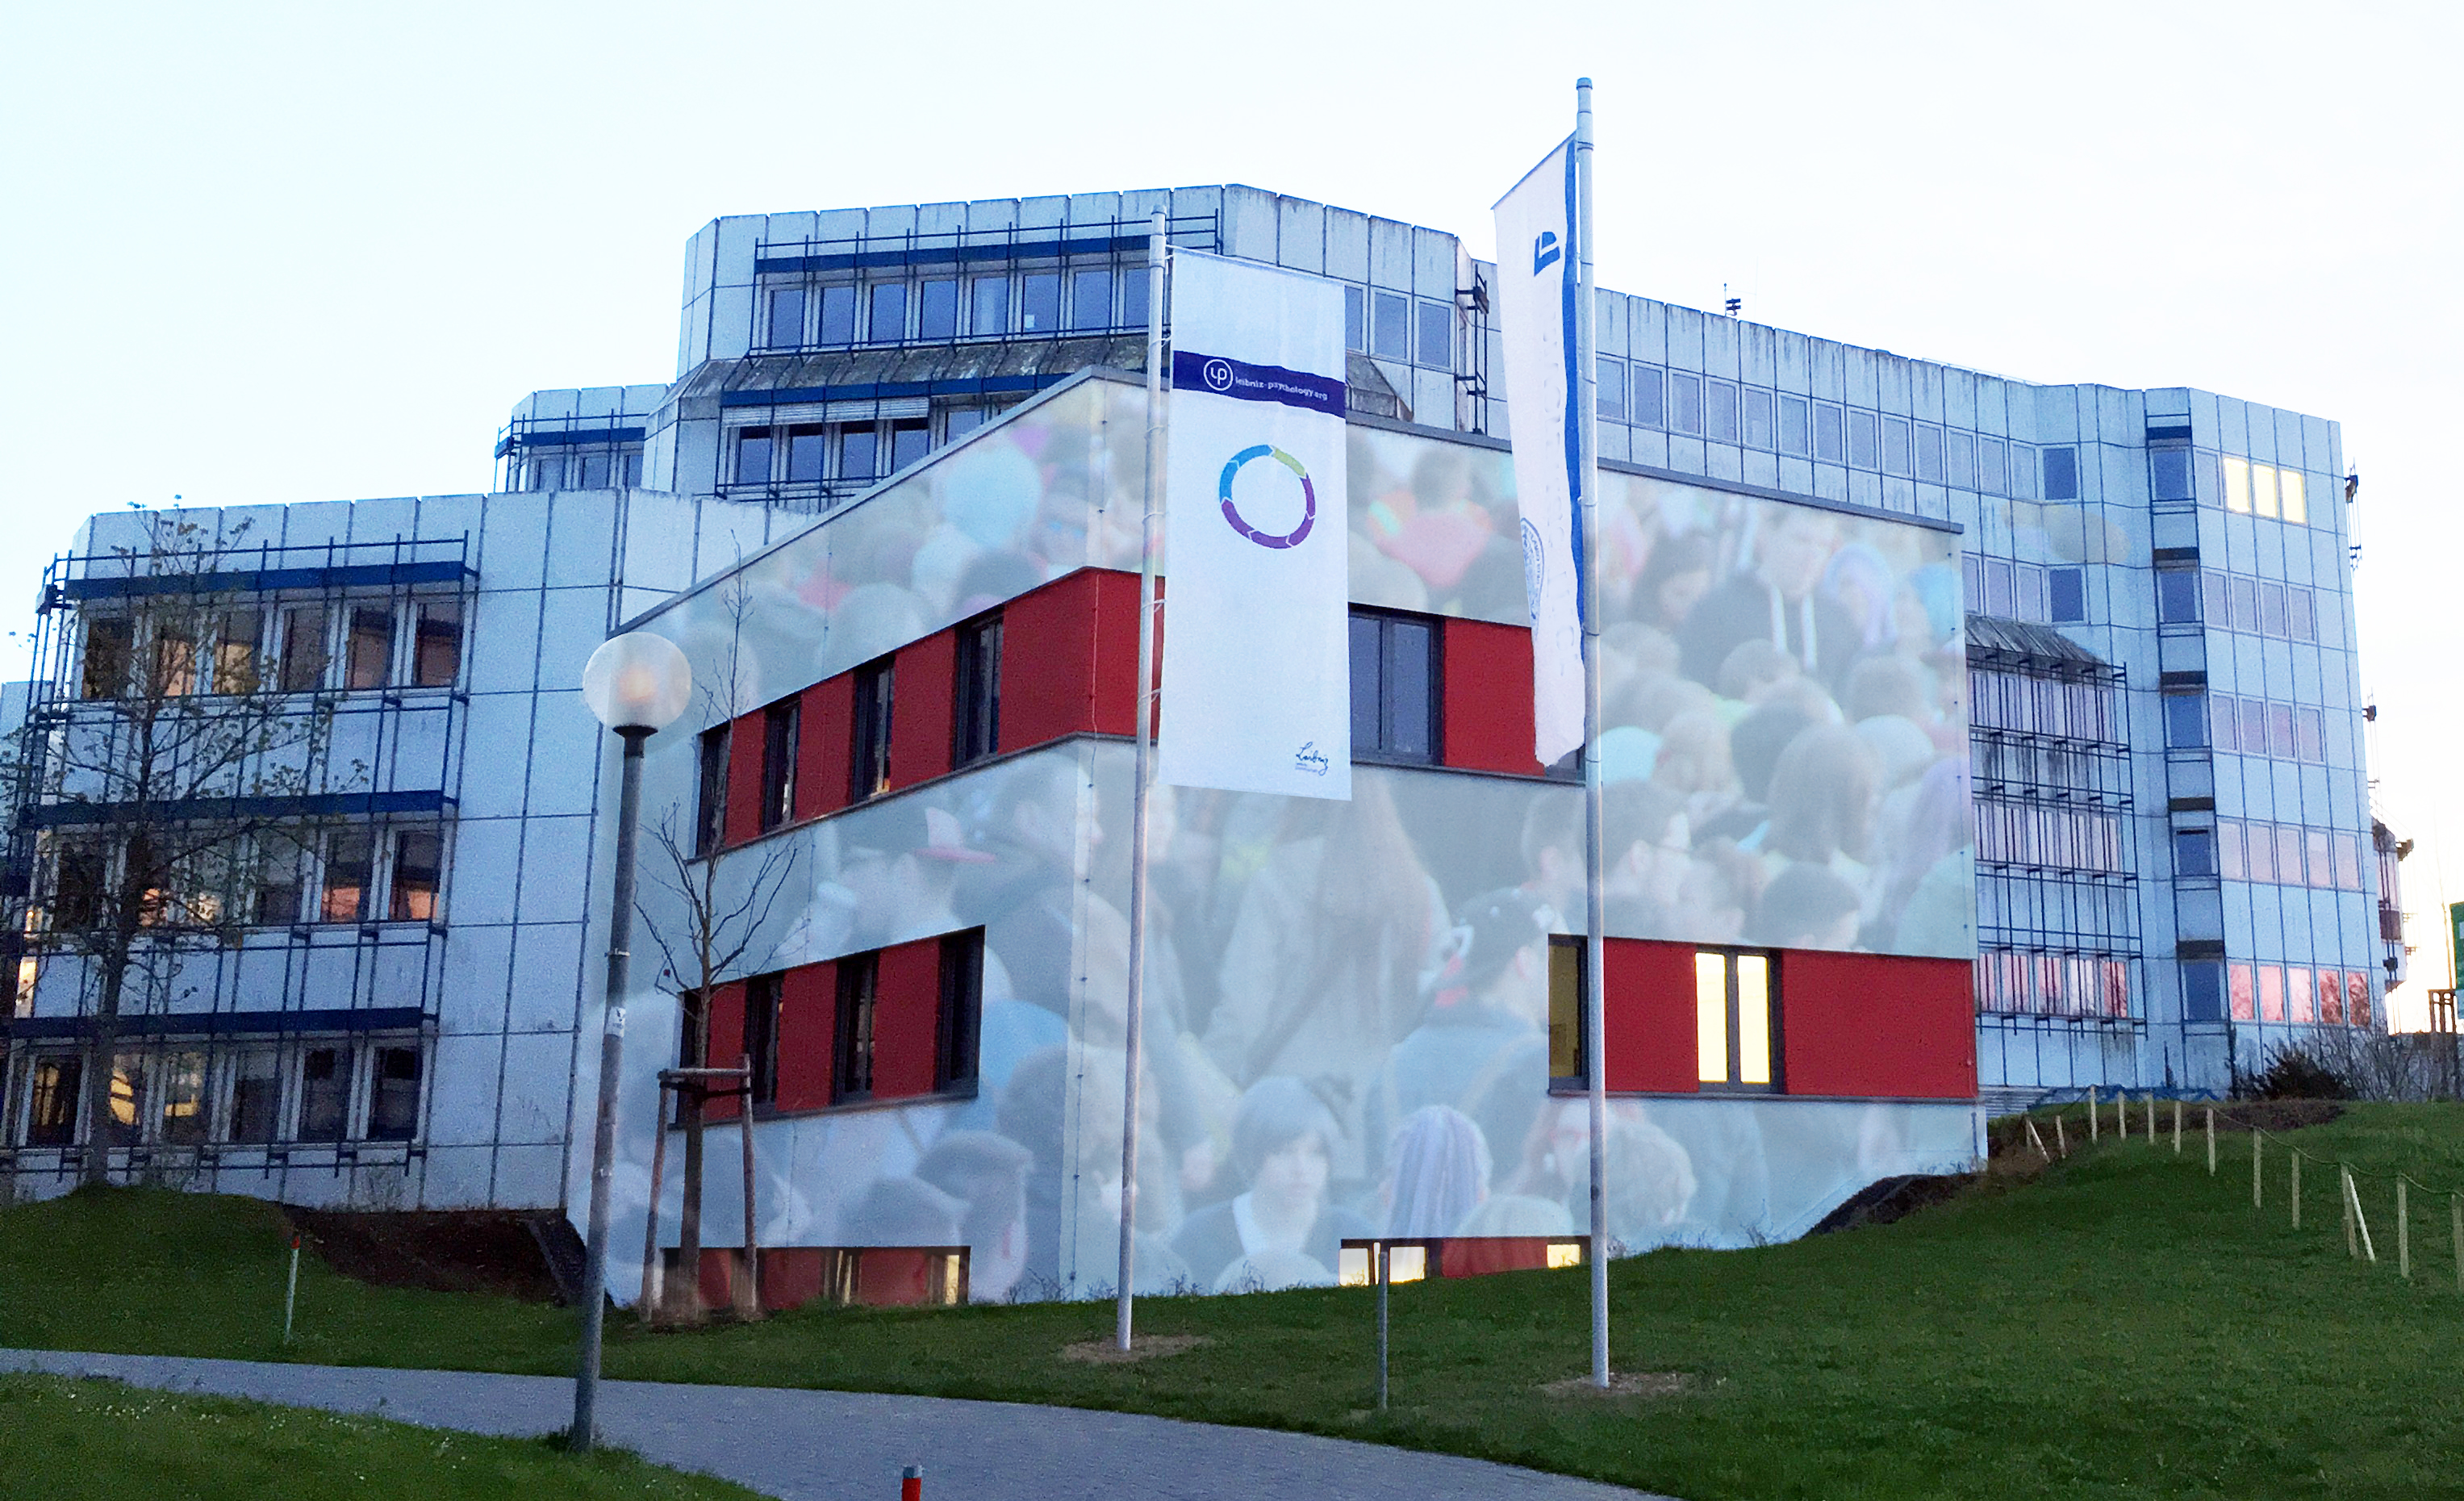
\includegraphics[width=0.8\linewidth]{3_Abbildungen/pfm_3_zpid_haus} \end{center}

\flushright
\tiny

\href{https://commons.wikimedia.org/w/index.php?curid=7048518}{Von
Mitchell 1985 - Eigenes Werk, CC BY-SA 4.0}
\end{frame}

\begin{frame}{Überblick}
\protect\hypertarget{uxfcberblick-5}{}
\textcolor{darkblue}{Das deutsche psychologische Dateninstitut}

\begin{center}
\includegraphics[width=0.65\linewidth]{3_Abbildungen/pfm_3_zpid} \end{center}
\end{frame}

\begin{frame}{Überblick}
\protect\hypertarget{uxfcberblick-6}{}
\textcolor{darkblue}{Psychologische Daten = Observierbare Variablen}
\vspace{1mm}

\begin{center}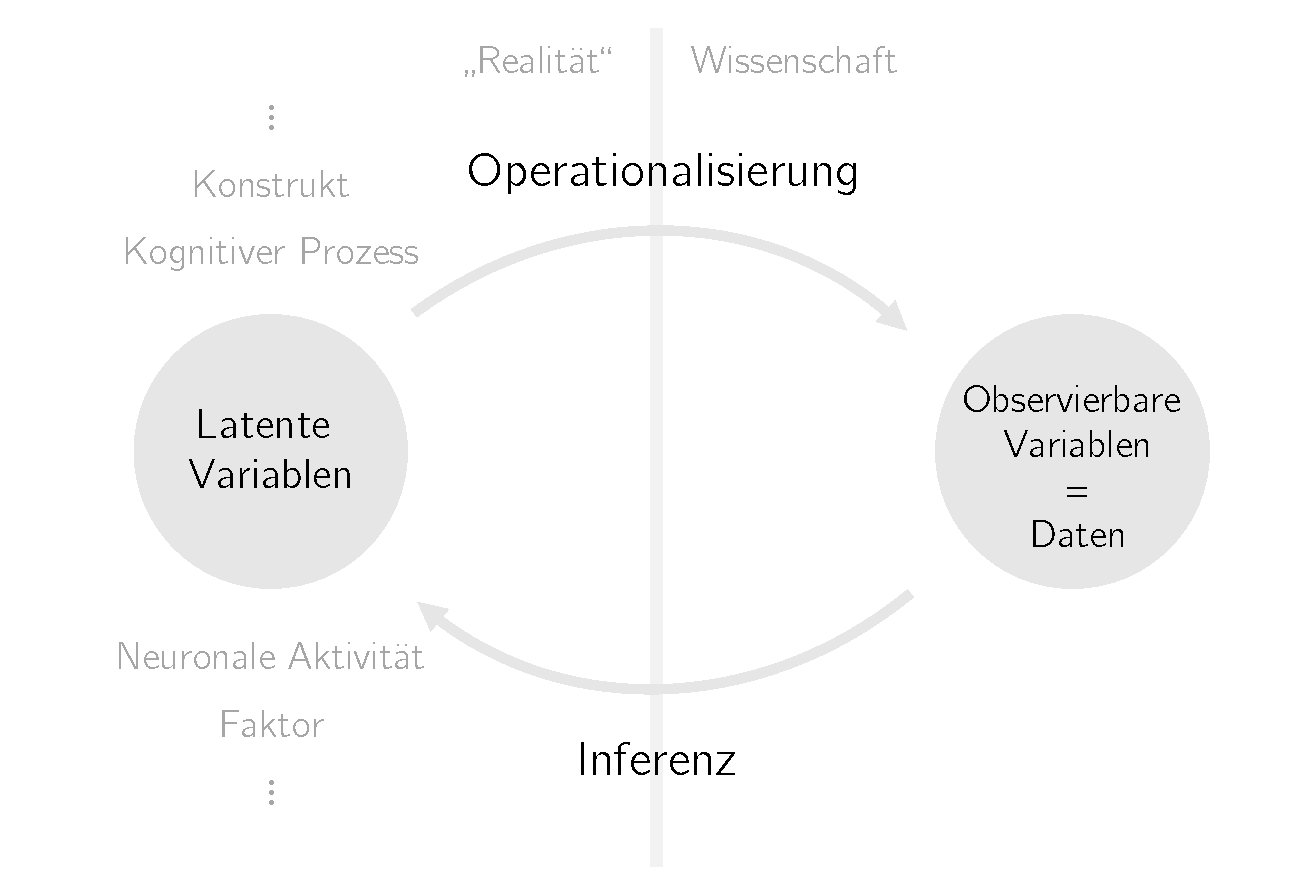
\includegraphics[width=0.85\linewidth]{3_Abbildungen/pfm_3_latente_variablen} \end{center}
\end{frame}

\begin{frame}{Überblick}
\protect\hypertarget{uxfcberblick-7}{}
\vspace{2mm}

\textcolor{darkblue}{Psychologische Datentypen} \vspace{-2mm}

\begin{center}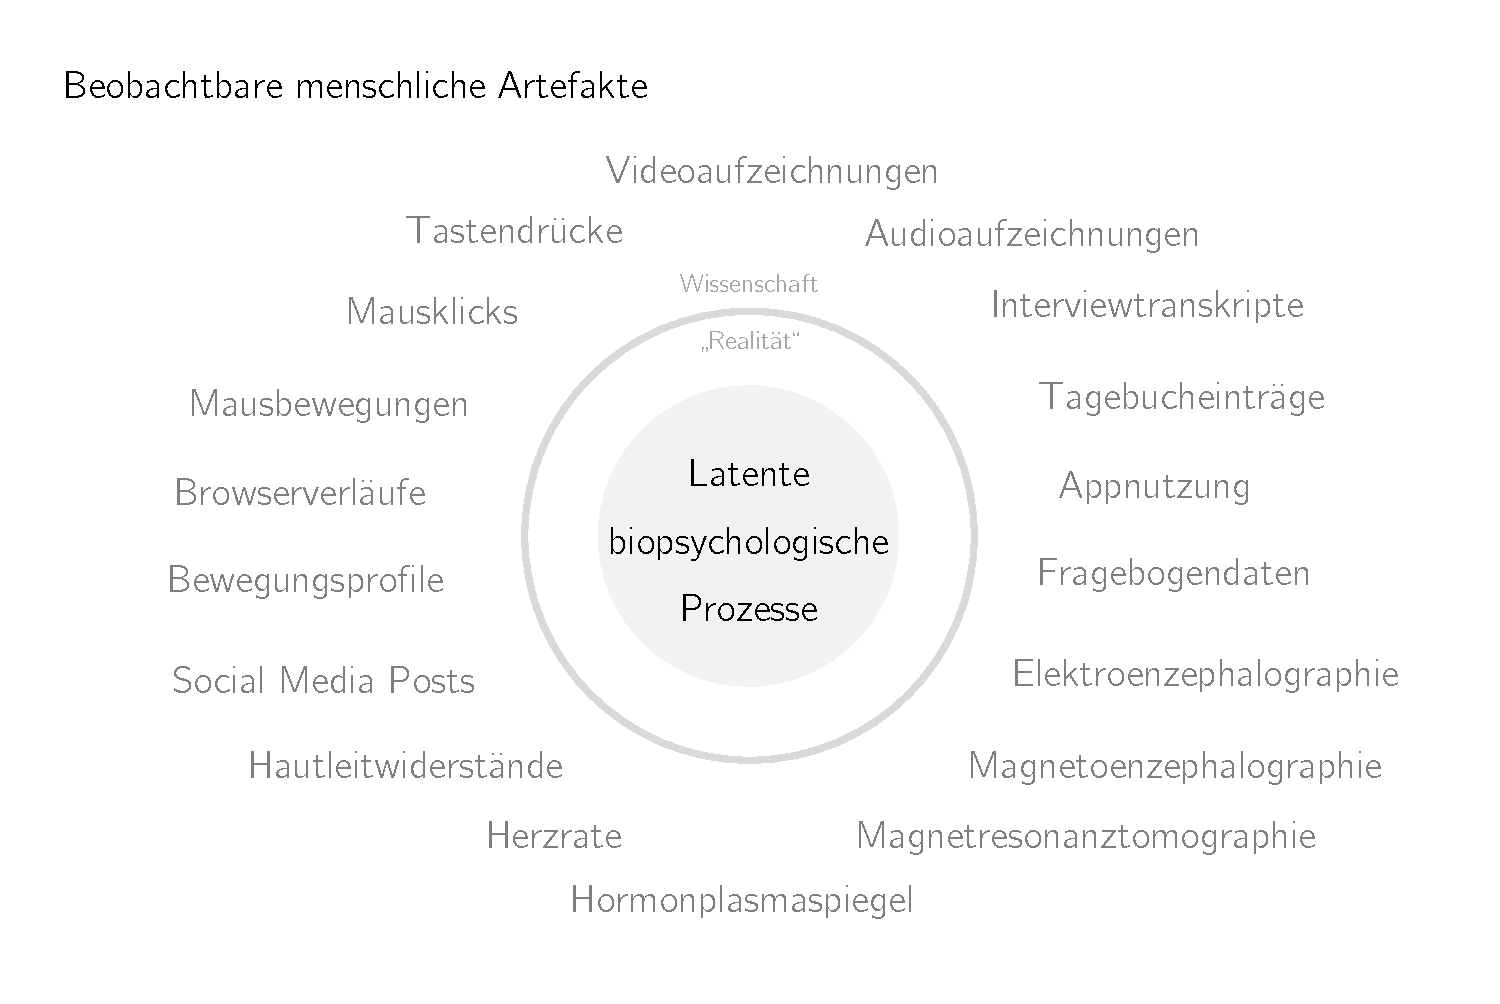
\includegraphics[width=1\linewidth]{3_Abbildungen/pfm_3_psychologische_daten} \end{center}
\end{frame}

\begin{frame}{Überblick}
\protect\hypertarget{uxfcberblick-8}{}
\textcolor{darkblue}{Datenaufnahmeraum} \vspace{-1mm}

\begin{center}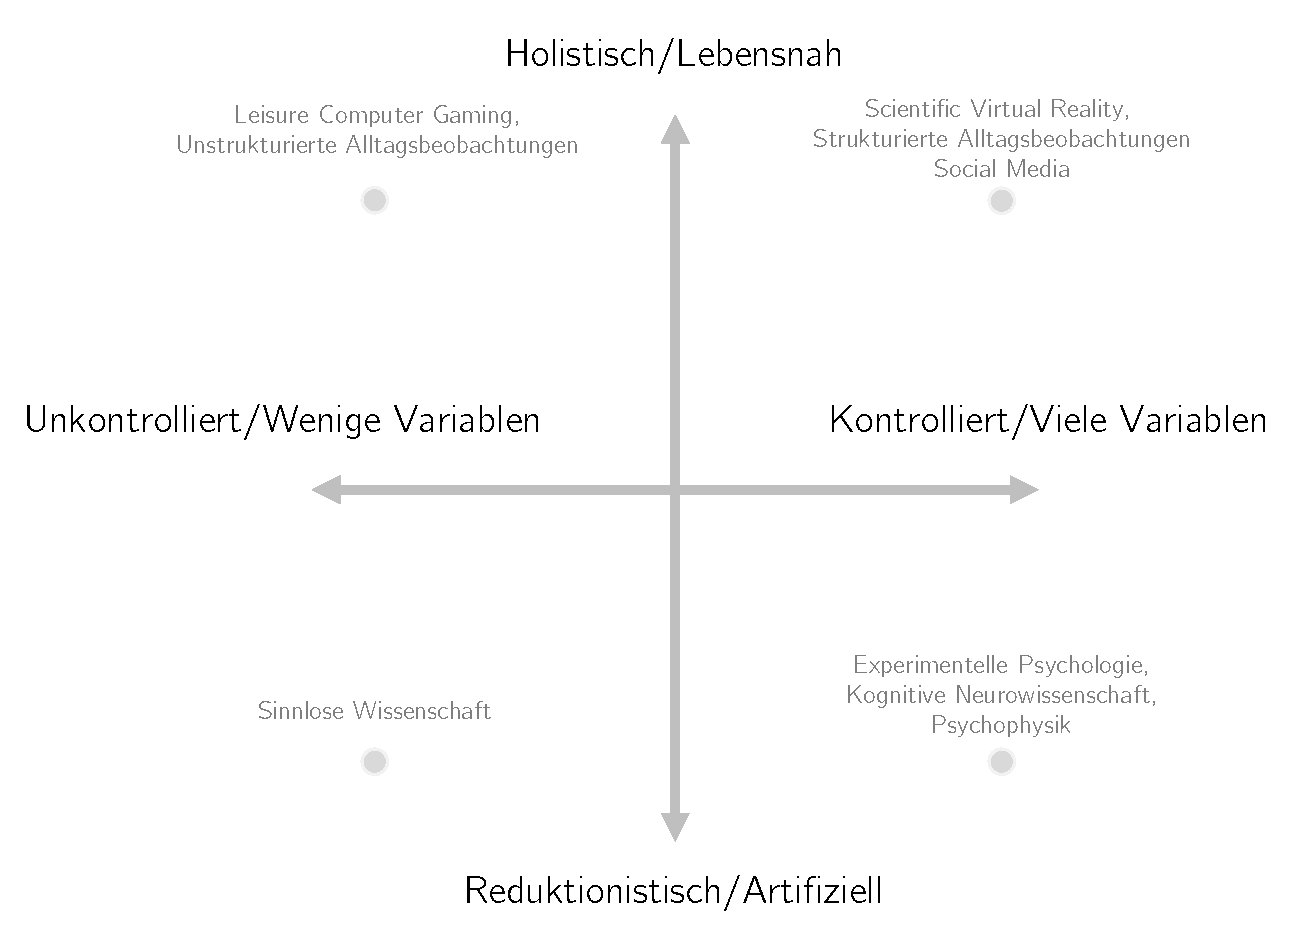
\includegraphics[width=0.85\linewidth]{3_Abbildungen/pfm_3_datenaufnahmeraum} \end{center}
\end{frame}

\begin{frame}{}
\protect\hypertarget{section-3}{}
\Large
\setstretch{3}
\vfill

Überblick

\textbf{Verhaltensdaten}

Physiologische Daten

Selbstkontrollfragen \vfill
\end{frame}

\begin{frame}{Verhaltensdaten}
\protect\hypertarget{verhaltensdaten}{}
\setstretch{1.7}

\textcolor{darkblue}{Beobachtungsdaten}

\begin{itemize}
\tightlist
\item
  Analoge strukturierte Fremdbeobachtung
\item
  Analoge strukturierte Selbstbeobachtung (Tagebucheinträge)
\item
  Digitale strukturierte Selbstbeobachtung (Ambulatory Assessment)
\item
  Computer-basierte Verhaltensparadigmen (Psychophysik,
  Verhaltenökonomie)
\item
  Computerspieldaten
\end{itemize}

\textcolor{darkblue}{Befragungsdaten}

\begin{itemize}
\tightlist
\item
  Mündliches Interview
\item
  Schriftliches Interview
\item
  Psychologische Tests und Fragebögen
\end{itemize}
\end{frame}

\begin{frame}{Verhaltensdaten}
\protect\hypertarget{verhaltensdaten-1}{}
Beobachtungsdaten \textbar{} Psychophysik und Verhaltensökonomie
\vspace{10mm}

\begin{center}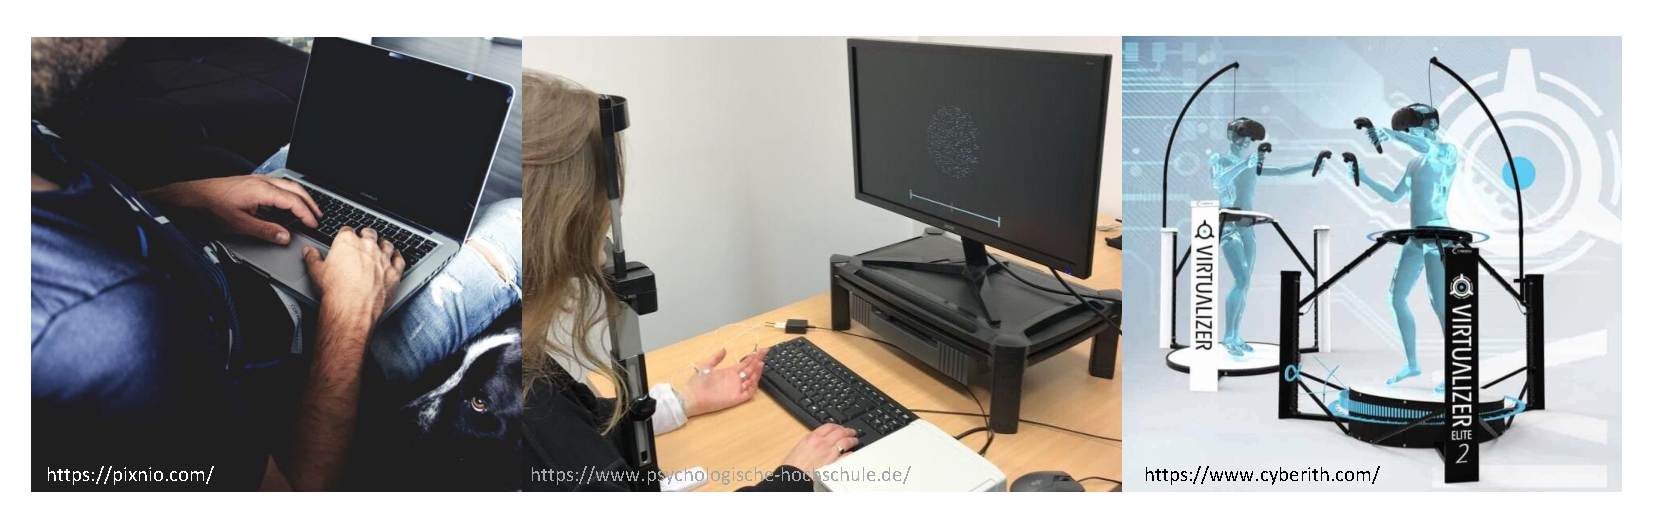
\includegraphics[width=1\linewidth]{3_Abbildungen/pfm_3_verhaltensdatenaufnahme} \end{center}
\end{frame}

\begin{frame}{Verhaltensdaten}
\protect\hypertarget{verhaltensdaten-2}{}
Beobachtungsdaten \textbar{} Psychophysik und Verhaltensökonomie

\small

Beispieldatensatz

\vspace{1mm}
\footnotesize

\(n = 8\) Proband:innen, \(m = 5\) binäre Entscheidungen, mögliche
Antworten als Elemente in \(\{0,1\}\) kodiert \vspace{1mm}

\begin{longtable}[]{@{}
  >{\raggedright\arraybackslash}p{(\columnwidth - 10\tabcolsep) * \real{0.1304}}
  >{\centering\arraybackslash}p{(\columnwidth - 10\tabcolsep) * \real{0.1739}}
  >{\centering\arraybackslash}p{(\columnwidth - 10\tabcolsep) * \real{0.1739}}
  >{\centering\arraybackslash}p{(\columnwidth - 10\tabcolsep) * \real{0.1739}}
  >{\centering\arraybackslash}p{(\columnwidth - 10\tabcolsep) * \real{0.1739}}
  >{\centering\arraybackslash}p{(\columnwidth - 10\tabcolsep) * \real{0.1739}}@{}}
\toprule()
\begin{minipage}[b]{\linewidth}\raggedright
\end{minipage} & \begin{minipage}[b]{\linewidth}\centering
Entscheidung 1
\end{minipage} & \begin{minipage}[b]{\linewidth}\centering
Entscheidung 2
\end{minipage} & \begin{minipage}[b]{\linewidth}\centering
Entscheidung 3
\end{minipage} & \begin{minipage}[b]{\linewidth}\centering
Entscheidung 4
\end{minipage} & \begin{minipage}[b]{\linewidth}\centering
Entscheidung 5
\end{minipage} \\
\midrule()
\endhead
Probandin 1 & 0 & 1 & 0 & 1 & 0 \\
Probandin 2 & 1 & 1 & 0 & 1 & 1 \\
Probandin 3 & 1 & 1 & 0 & 0 & 0 \\
Probandin 4 & 0 & 0 & 1 & 1 & 0 \\
Probandin 5 & 0 & 0 & 0 & 1 & 1 \\
Probandin 6 & 0 & 0 & 1 & 1 & 1 \\
Probandin 7 & 0 & 0 & 1 & 0 & 0 \\
Probandin 8 & 0 & 0 & 0 & 0 & 0 \\
\bottomrule()
\end{longtable}
\end{frame}

\begin{frame}{Verhaltensdaten}
\protect\hypertarget{verhaltensdaten-3}{}
Befragungsdaten \textbar{} Psychologische Tests und Fragebögen
\vspace{-2mm}

\begin{center}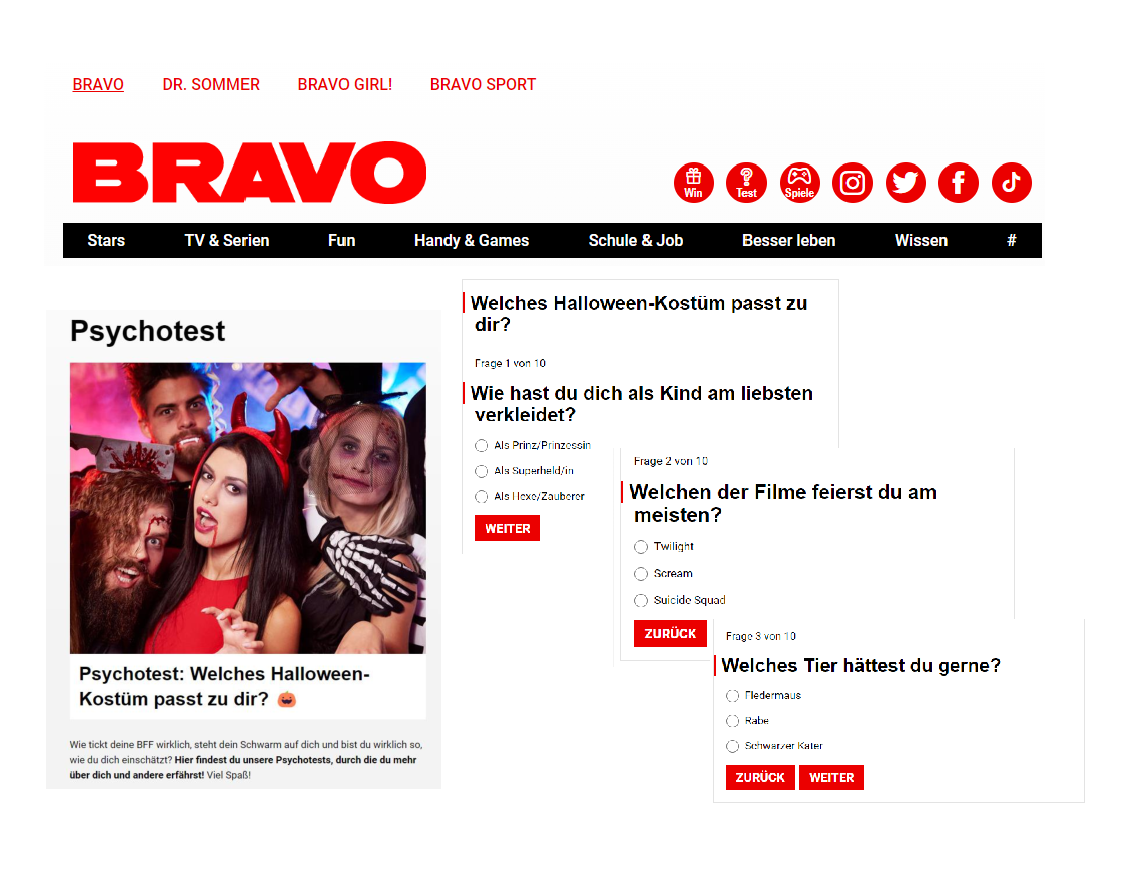
\includegraphics[width=0.75\linewidth]{3_Abbildungen/pfm_3_fragebogen_1} \end{center}
\end{frame}

\begin{frame}{Verhaltendaten}
\protect\hypertarget{verhaltendaten}{}
\vspace{1mm}

Befragungsdaten \textbar{} Psychologische Tests und Fragebögen
\vspace{-3mm}

\begin{center}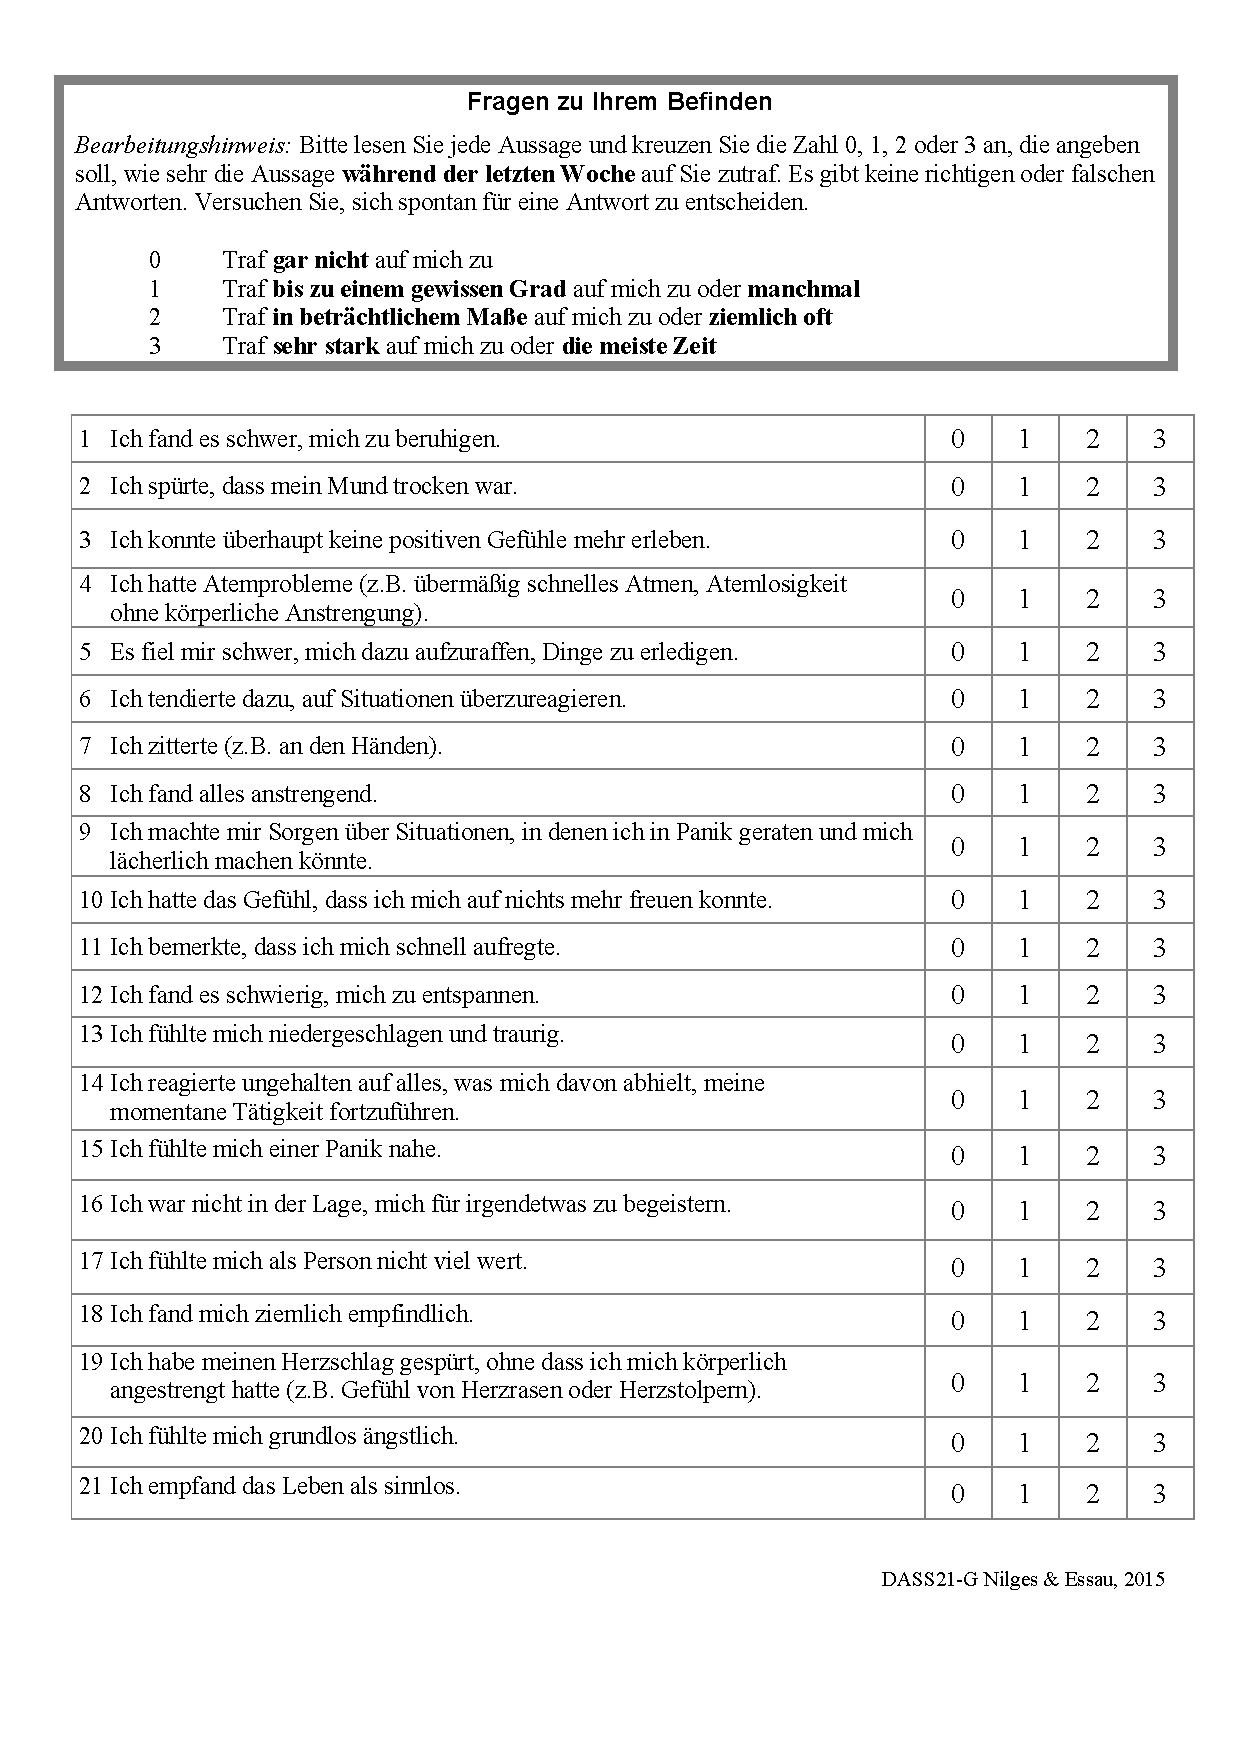
\includegraphics[width=0.4\linewidth]{3_Abbildungen/pfm_3_fragebogen_2} \end{center}
\vspace{-3mm}
\flushright
\tiny

Nilges, P. \& Essau, C. (2021). DASS. Depressions-Angst-Stress-Skalen -
deutschsprachige Kurzfassung {[}Verfahrensdokumentation und Fragebogen
mit Auswertung{]}. In Leibniz-Institut für Psychologie (ZPID) (Hrsg.),
Open Test Archive. Trier: ZPID.
\url{https://doi.org/10.23668/psycharchives.4579}
\end{frame}

\begin{frame}{Verhaltensdaten}
\protect\hypertarget{verhaltensdaten-4}{}
Befragungsdaten \textbar{} Psychologische Tests und Fragebögen

\small

Beispieldatensatz

\footnotesize
\vspace{1mm}

\(n = 8\) Proband:innen, \(m = 5\) Fragen, mögliche Antworten als
Elemente in \(\mathbb{N}_7\) kodiert \vspace{1mm}

\begin{longtable}[]{@{}lccccc@{}}
\toprule()
& Frage 1 & Frage 2 & Frage 3 & Frage 4 & Frage 5 \\
\midrule()
\endhead
Proband:in 1 & 5 & 7 & 2 & 5 & 1 \\
Proband:in 2 & 4 & 3 & 5 & 2 & 4 \\
Proband:in 3 & 5 & 4 & 1 & 7 & 3 \\
Proband:in 4 & 5 & 3 & 3 & 4 & 1 \\
Proband:in 5 & 2 & 2 & 6 & 4 & 3 \\
Proband:in 6 & 6 & 4 & 3 & 3 & 4 \\
Proband:in 7 & 6 & 4 & 4 & 4 & 6 \\
Proband:in 8 & 7 & 6 & 3 & 3 & 3 \\
\bottomrule()
\end{longtable}
\end{frame}

\begin{frame}{}
\protect\hypertarget{section-4}{}
\Large
\setstretch{3}
\vfill

Überblick

Verhaltensdaten

\textbf{Physiologische Daten}

Selbstkontrollfragen \vfill
\end{frame}

\begin{frame}{Physiologische Daten}
\protect\hypertarget{physiologische-daten}{}
\setstretch{1.8}

\textcolor{darkblue}{Vegetativphysiologische Daten}

\begin{itemize}
\tightlist
\item
  Medizinische Befunde
\item
  Hormonspiegel
\item
  Immunmarker
\item
  Hautleitwiderstand
\end{itemize}

\textcolor{darkblue}{Neurophysiologische Daten}

\begin{itemize}
\tightlist
\item
  Elektroenzephalographie (EEG)
\item
  Magnetoenzephalographie (MEG)
\item
  Funktionelle Magnetresonanztomographie (fMRT)
\item
  Magnet- und Gleichstromstimulationsverfahren (TMS, tCDS)
\end{itemize}
\end{frame}

\begin{frame}{Physiologische Daten}
\protect\hypertarget{physiologische-daten-1}{}
Vegetativphysiologische Daten \textbar{} Hautleitwiderstand\\
\vspace{5mm}

\begin{center}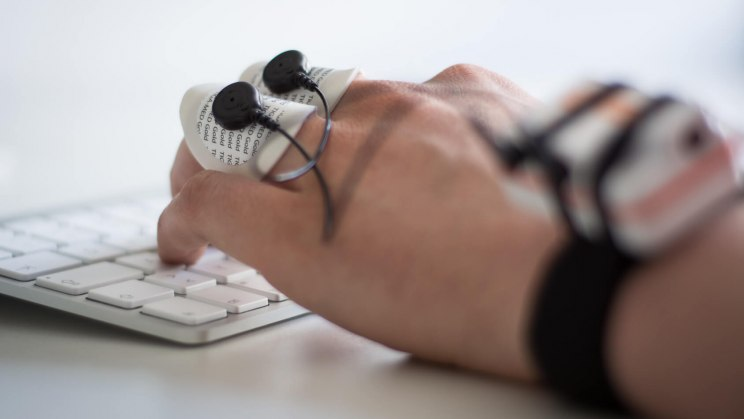
\includegraphics[width=0.75\linewidth]{3_Abbildungen/pfm_3_hautleitwiderstand} \end{center}
\end{frame}

\begin{frame}{Physiologische Daten}
\protect\hypertarget{physiologische-daten-2}{}
Vegetativphysiologische Daten \textbar{} Hautleitwiderstand

\small

Beispieldatensatz

\footnotesize
\vspace{1mm}

\(1\) Fingerelektrode, \(n = 8\) Proband:innen, \(m = 7\) Messzeitpunkte
(2 ms), mögliche Werte in \(\mathbb{R}\) (\(\mu V\)) kodiert
\vspace{1mm}

\begin{longtable}[]{@{}lccccccc@{}}
\toprule()
& 0 ms & 2 ms & 4 ms & 6 ms & 8 ms & 10 ms & 12 ms \\
\midrule()
\endhead
Proband:in 1 & 5.75 & 7.05 & 5.92 & 4.76 & 1.10 & 8.73 & 2.08 \\
Proband:in 2 & 6.41 & 1.53 & 8.51 & 7.02 & 8.99 & 6.10 & 2.75 \\
Proband:in 3 & 3.35 & 9.97 & 1.25 & 5.57 & 9.97 & 3.28 & 2.48 \\
Proband:in 4 & 3.61 & 2.34 & 5.22 & 6.94 & 5.50 & 9.27 & 6.97 \\
Proband:in 5 & 5.32 & 5.67 & 8.25 & 5.61 & 4.23 & 8.81 & 8.71 \\
Proband:in 6 & 9.28 & 8.62 & 8.33 & 8.52 & 7.97 & 3.24 & 9.34 \\
Proband:in 7 & 4.61 & 7.46 & 4.63 & 7.38 & 6.26 & 4.63 & 5.97 \\
Proband:in 8 & 2.92 & 3.17 & 2.97 & 8.87 & 6.71 & 7.93 & 6.19 \\
\bottomrule()
\end{longtable}
\end{frame}

\begin{frame}{Physiologische Daten}
\protect\hypertarget{physiologische-daten-3}{}
Neurophysiologische Daten \textbar{} EEG \vspace{5mm}

\begin{center}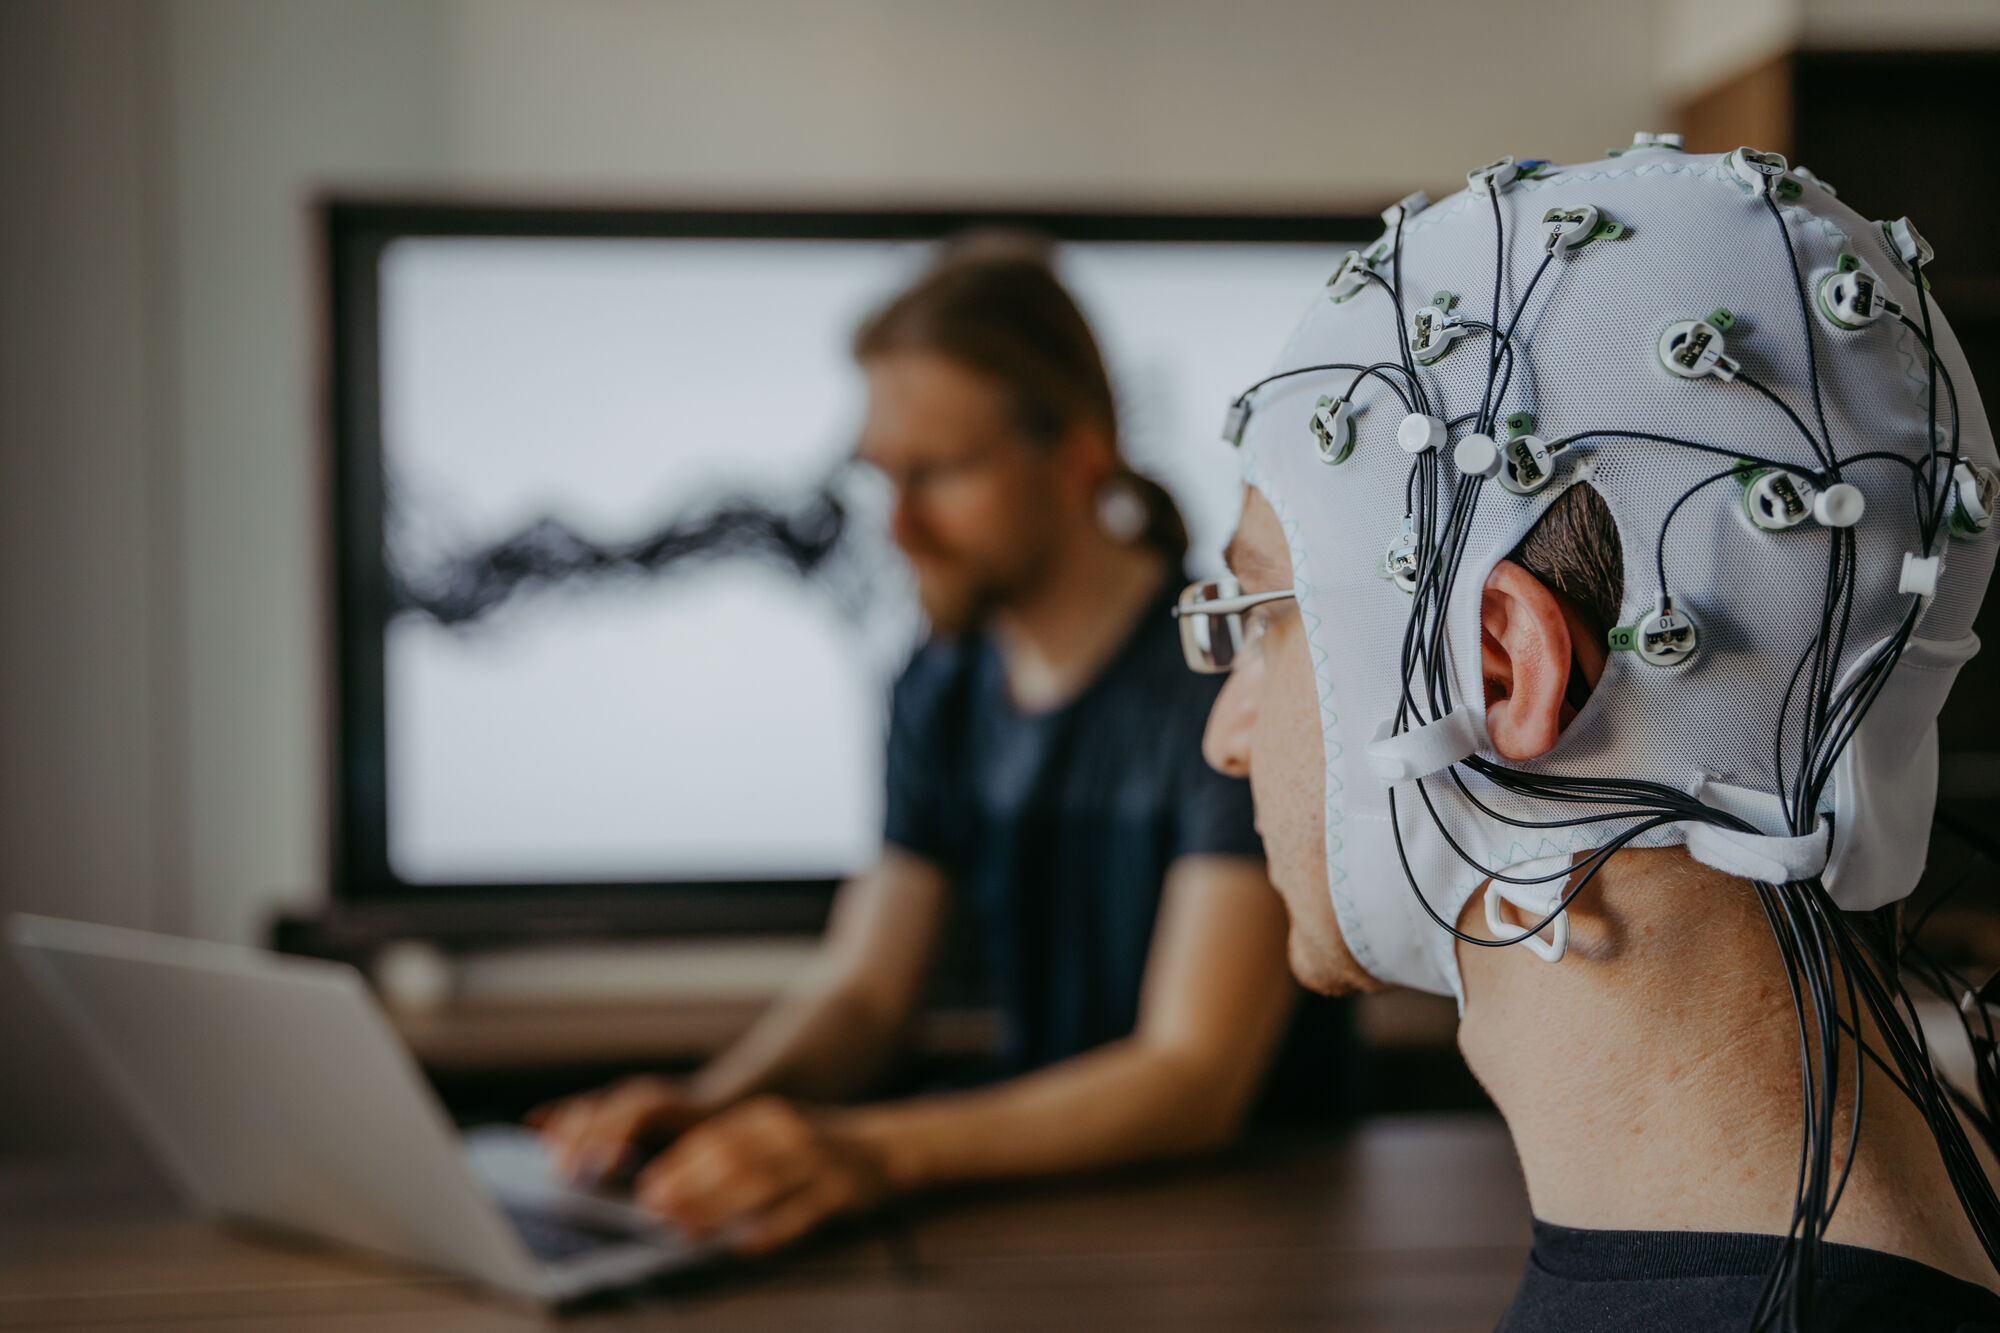
\includegraphics[width=0.7\linewidth]{3_Abbildungen/pfm_3_eeg} \end{center}
\end{frame}

\begin{frame}{Physiologische Daten}
\protect\hypertarget{physiologische-daten-4}{}
Neurophysiologische Daten \textbar{} EEG

\begin{center}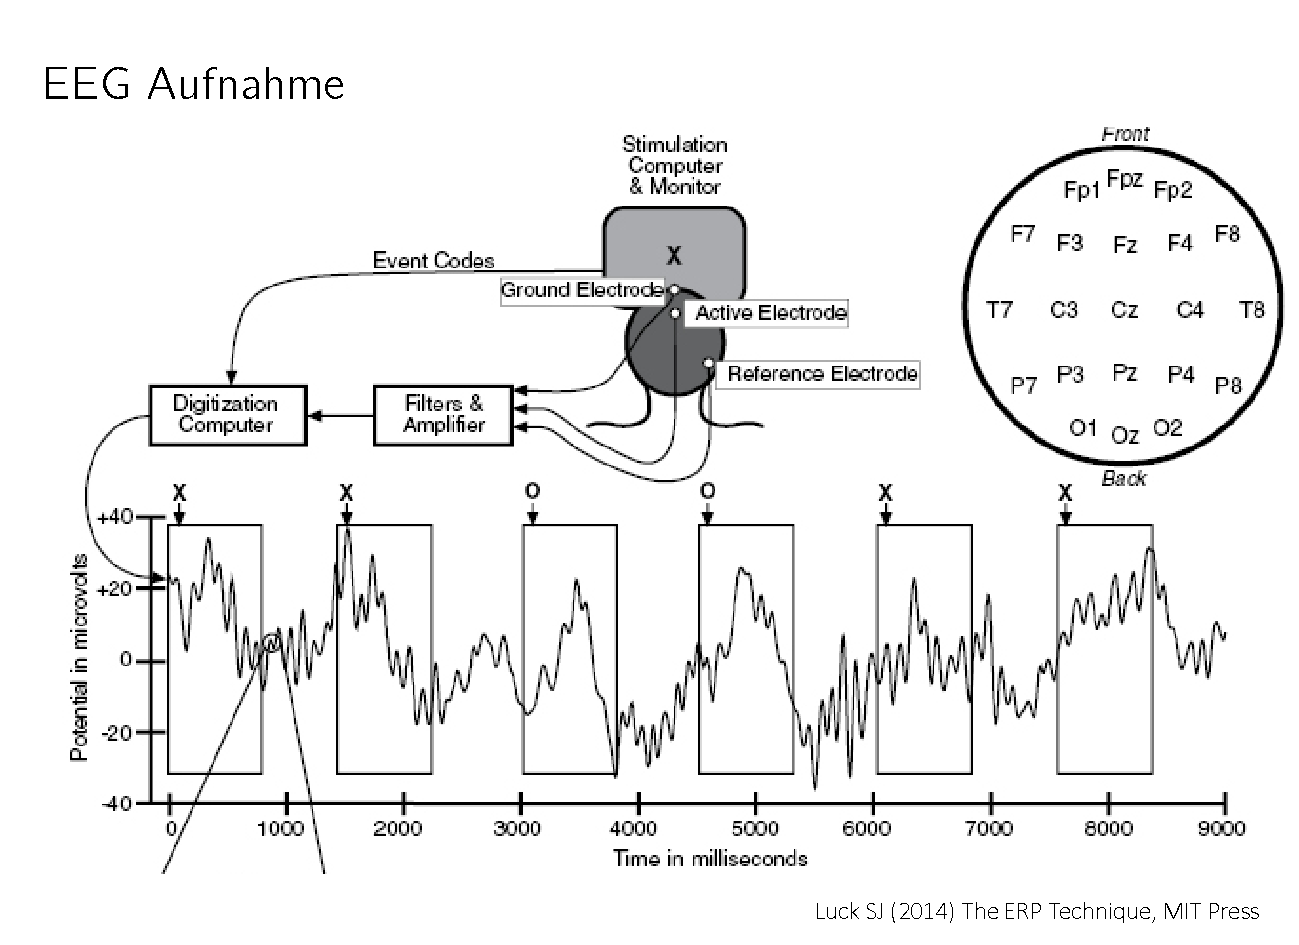
\includegraphics[width=0.8\linewidth]{3_Abbildungen/pfm_3_eeg_aufnahme} \end{center}
\end{frame}

\begin{frame}{Physiologische Daten}
\protect\hypertarget{physiologische-daten-5}{}
Neurophysiologische Daten \textbar{} EEG

\begin{center}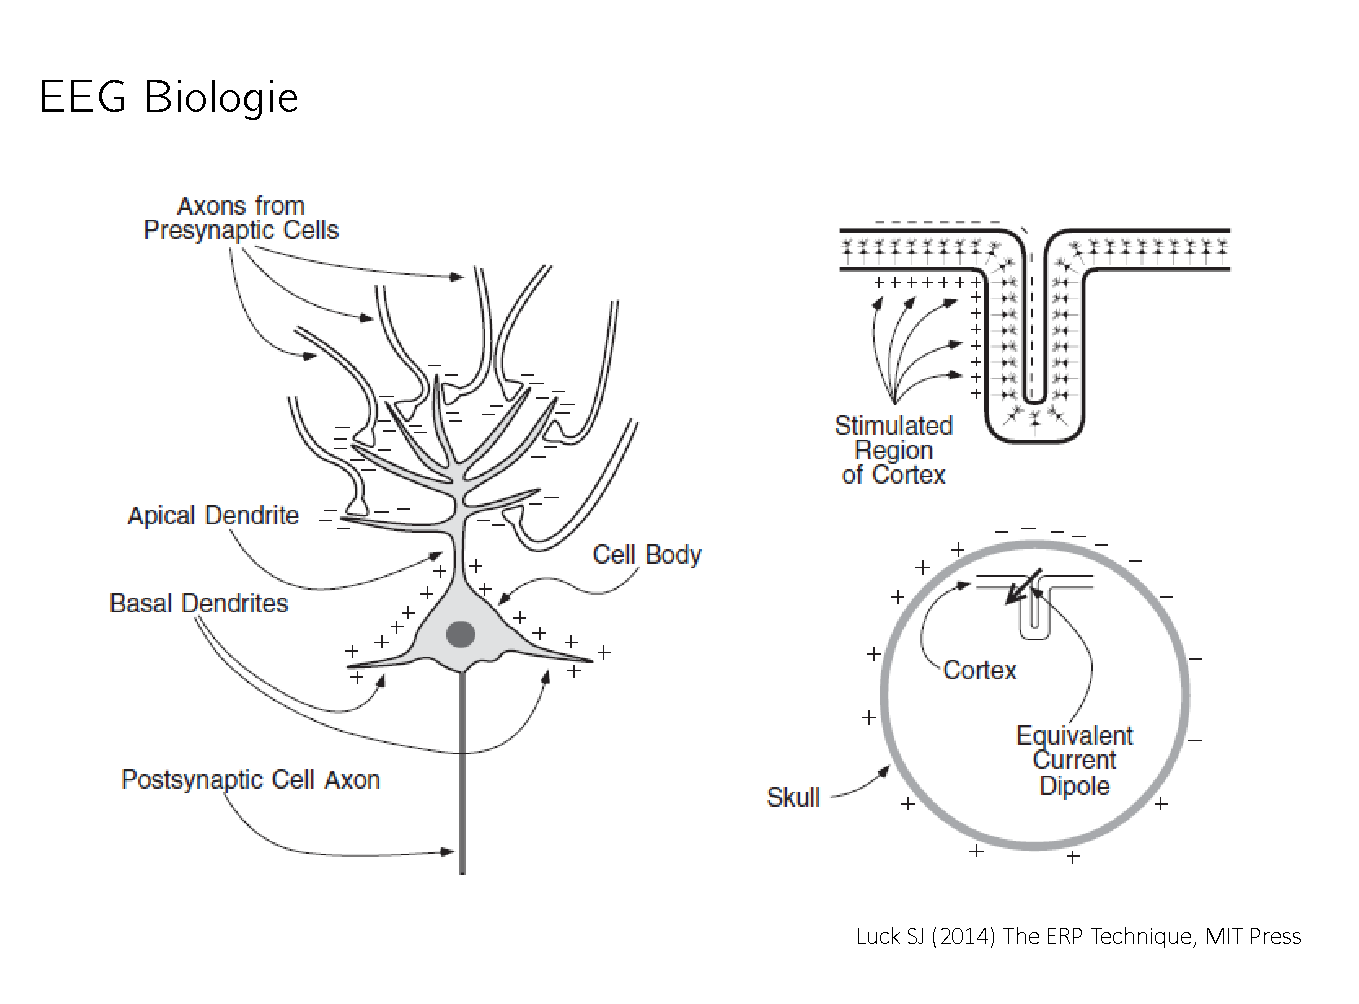
\includegraphics[width=0.8\linewidth]{3_Abbildungen/pfm_3_eeg_biologie} \end{center}
\end{frame}

\begin{frame}{Physiologische Daten}
\protect\hypertarget{physiologische-daten-6}{}
Neurophysiologische Daten \textbar{} EEG

\small

Beispieldatensatz

\footnotesize
\vspace{1mm}

\(1\) Proband:in, \(n = 8\) Elektroden, \(m = 7\) Messzeitpunkte (2 ms),
mögliche Werte in \(\mathbb{R}\) (\(\mu V\)) kodiert \vspace{1mm}

\begin{longtable}[]{@{}
  >{\raggedright\arraybackslash}p{(\columnwidth - 14\tabcolsep) * \real{0.1818}}
  >{\centering\arraybackslash}p{(\columnwidth - 14\tabcolsep) * \real{0.1212}}
  >{\centering\arraybackslash}p{(\columnwidth - 14\tabcolsep) * \real{0.1212}}
  >{\centering\arraybackslash}p{(\columnwidth - 14\tabcolsep) * \real{0.1061}}
  >{\centering\arraybackslash}p{(\columnwidth - 14\tabcolsep) * \real{0.1061}}
  >{\centering\arraybackslash}p{(\columnwidth - 14\tabcolsep) * \real{0.1212}}
  >{\centering\arraybackslash}p{(\columnwidth - 14\tabcolsep) * \real{0.1212}}
  >{\centering\arraybackslash}p{(\columnwidth - 14\tabcolsep) * \real{0.1212}}@{}}
\toprule()
\begin{minipage}[b]{\linewidth}\raggedright
\end{minipage} & \begin{minipage}[b]{\linewidth}\centering
0 ms
\end{minipage} & \begin{minipage}[b]{\linewidth}\centering
2 ms
\end{minipage} & \begin{minipage}[b]{\linewidth}\centering
4 ms
\end{minipage} & \begin{minipage}[b]{\linewidth}\centering
6 ms
\end{minipage} & \begin{minipage}[b]{\linewidth}\centering
8 ms
\end{minipage} & \begin{minipage}[b]{\linewidth}\centering
10 ms
\end{minipage} & \begin{minipage}[b]{\linewidth}\centering
12 ms
\end{minipage} \\
\midrule()
\endhead
Elektrode 1 & 6.249 & 8.913 & 6.736 & 9.674 & 1.501 & 6.014 & 8.234 \\
Elektrode 2 & 0.937 & -1.551 & 0.605 & 7.829 & 6.661 & 2.896 & -0.724 \\
Elektrode 3 & -1.465 & 5.123 & 3.475 & 8.835 & 8.399 & 2.215 & 3.818 \\
Elektrode 4 & 8.918 & 0.844 & 1.994 & 4.976 & 0.861 & 6.857 & 0.967 \\
Elektrode 5 & -1.152 & 8.876 & 4.820 & 7.276 & -1.946 & 5.971 & 6.239 \\
Elektrode 6 & 9.963 & 7.826 & 1.026 & 9.941 & 9.322 & -0.977 & -0.037 \\
Elektrode 7 & 5.342 & 6.398 & 3.568 & 6.532 & 3.258 & 8.274 & 9.434 \\
Elektrode 8 & 0.071 & 0.640 & 9.012 & 0.579 & 7.007 & -1.076 & 1.862 \\
\bottomrule()
\end{longtable}
\end{frame}

\begin{frame}{Physiologische Daten}
\protect\hypertarget{physiologische-daten-7}{}
Neurophysiologische Daten \textbar{} fMRT \vspace{5mm}

\begin{center}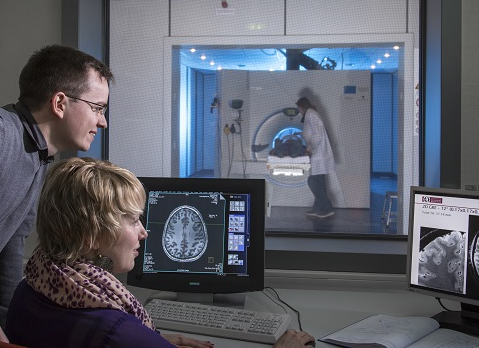
\includegraphics[width=0.7\linewidth]{3_Abbildungen/pfm_3_fmrt} \end{center}
\end{frame}

\begin{frame}{Physiologische Daten}
\protect\hypertarget{physiologische-daten-8}{}
Neurophysiologische Daten \textbar{} fMRT \vspace{1mm}

\begin{center}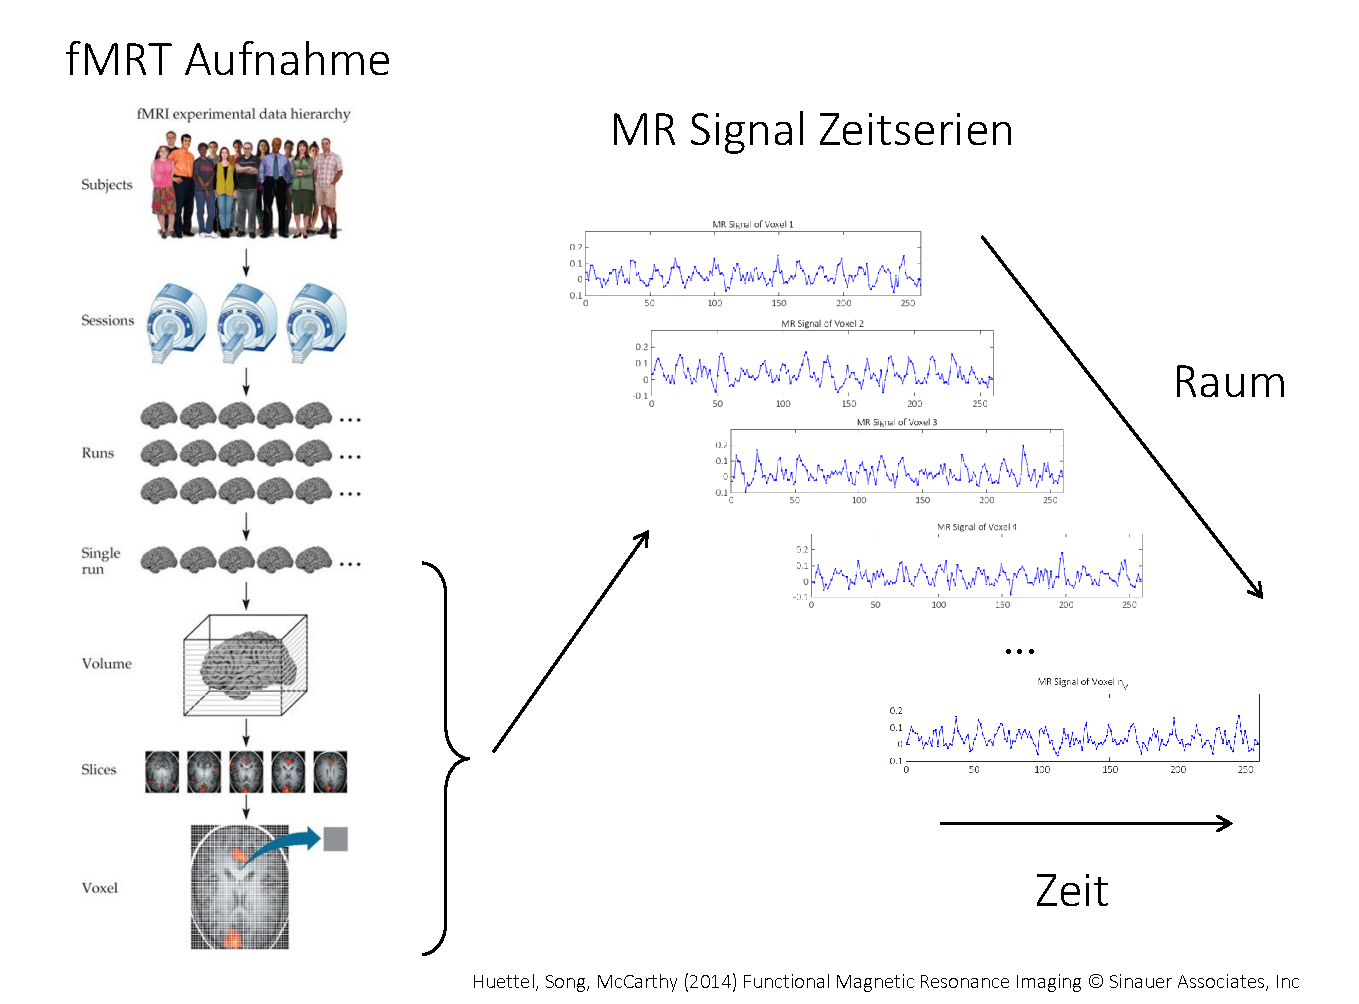
\includegraphics[width=0.8\linewidth]{3_Abbildungen/pfm_3_fmrt_aufnahme} \end{center}
\end{frame}

\begin{frame}{Physiologische Daten}
\protect\hypertarget{physiologische-daten-9}{}
Neurophysiologische Daten \textbar{} fMRT \vspace{3mm}

\begin{center}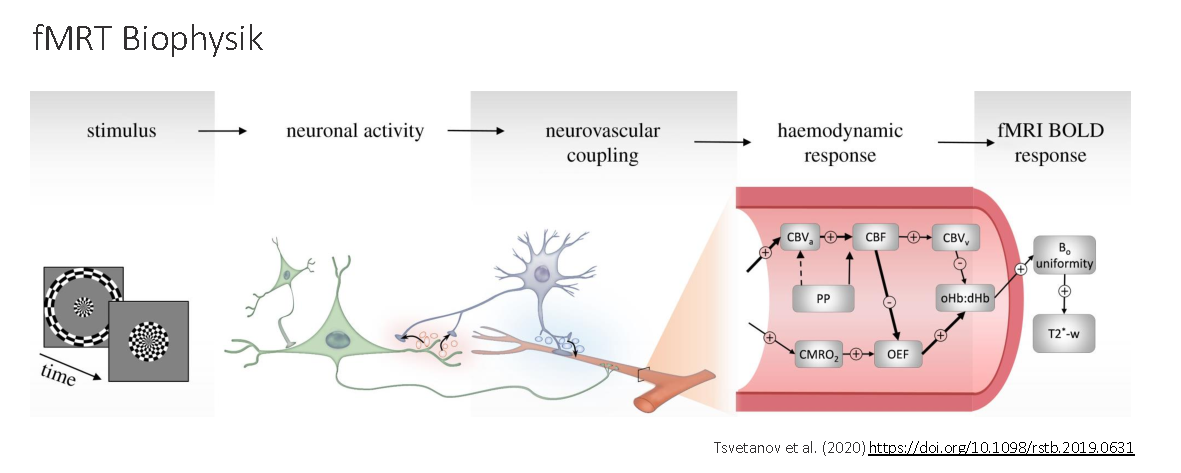
\includegraphics[width=0.9\linewidth]{3_Abbildungen/pfm_3_fmrt_biophysik} \end{center}
\end{frame}

\begin{frame}{Physiologische Daten}
\protect\hypertarget{physiologische-daten-10}{}
Neurophysiologische Daten \textbar{} fMRT

\small

Beispieldatensatz

\footnotesize
\vspace{1mm}

\(1\) Proband:in, \(n = 8\) Voxel, \(m = 7\) Messzeitpunkte (1.5 s),
mögliche Werte in \(\mathbb{N}_{255}\) kodiert \vspace{1mm}

\begin{longtable}[]{@{}lccccccc@{}}
\toprule()
& 0 s & 1.5 s & 3 s & 4.5 s & 6 s & 7.5 s & 9 s \\
\midrule()
\endhead
Voxel 1 & 92 & 89 & 10 & 150 & 154 & 169 & 250 \\
Voxel 2 & 226 & 242 & 241 & 194 & 168 & 99 & 4 \\
Voxel 3 & 211 & 55 & 62 & 213 & 84 & 12 & 172 \\
Voxel 4 & 26 & 8 & 199 & 195 & 250 & 157 & 95 \\
Voxel 5 & 231 & 37 & 74 & 106 & 182 & 153 & 234 \\
Voxel 6 & 197 & 218 & 223 & 35 & 223 & 104 & 173 \\
Voxel 7 & 98 & 54 & 75 & 21 & 251 & 219 & 170 \\
Voxel 8 & 255 & 54 & 251 & 167 & 56 & 132 & 193 \\
\bottomrule()
\end{longtable}
\end{frame}

\begin{frame}{Überblick}
\protect\hypertarget{uxfcberblick-9}{}
\vspace{2mm}

\textcolor{darkblue}{Psychologische Datentypen} \vspace{-2mm}

\begin{center}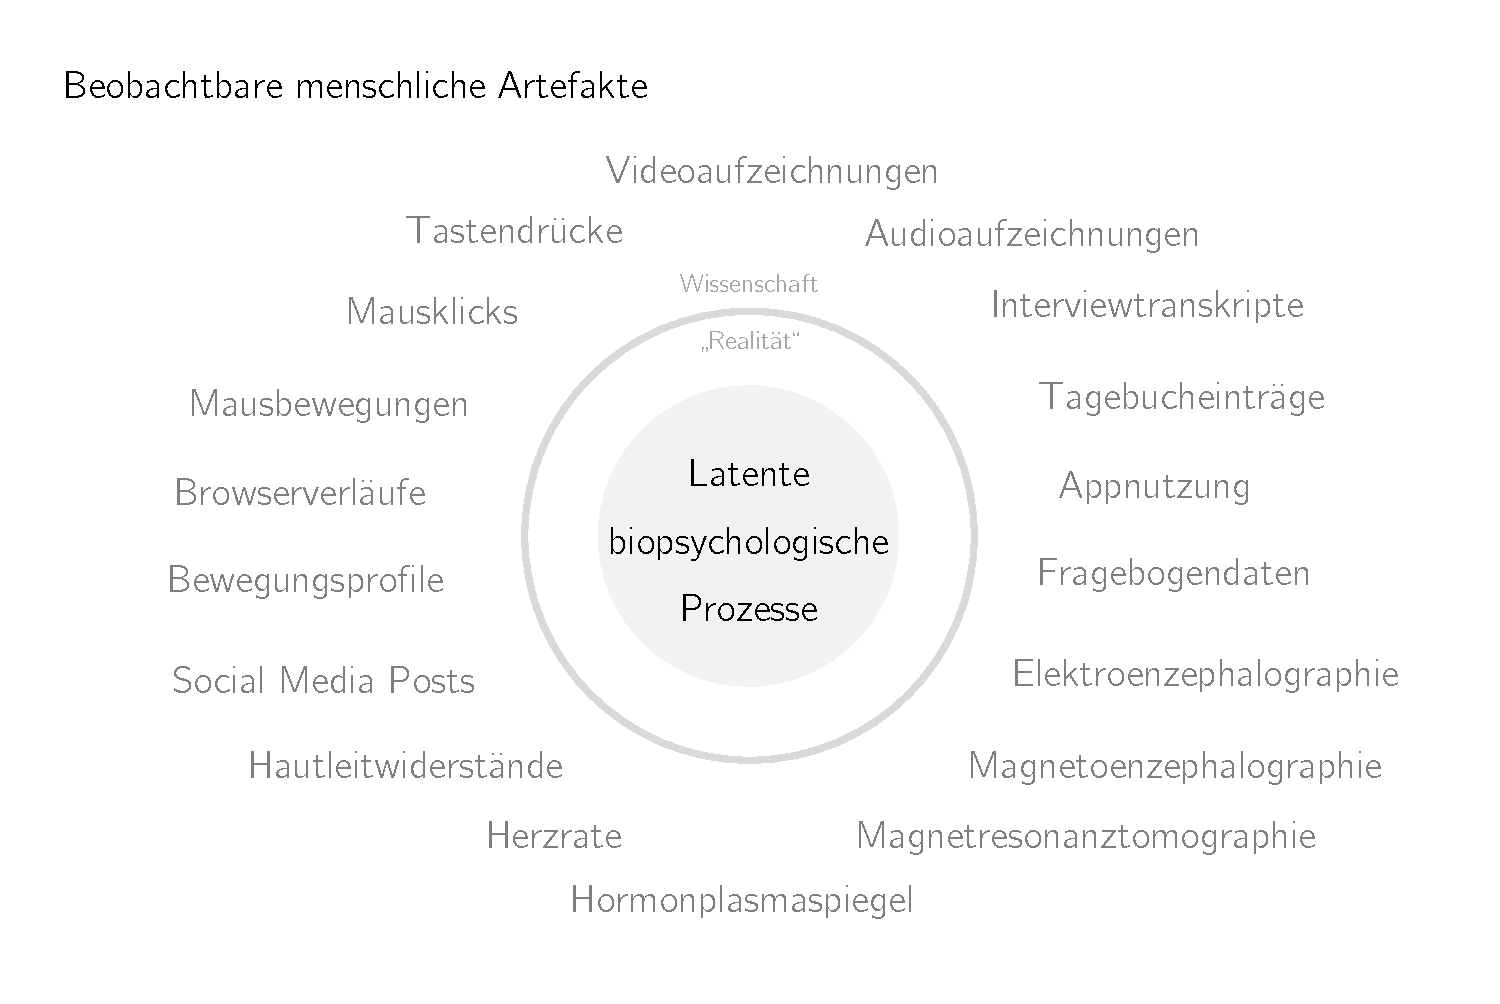
\includegraphics[width=1\linewidth]{3_Abbildungen/pfm_3_psychologische_daten} \end{center}
\end{frame}

\begin{frame}{}
\protect\hypertarget{section-5}{}
\Large
\setstretch{3}
\vfill

Überblick

Verhaltensdaten

Physiologische Daten

\textbf{Selbstkontrollfragen} \vfill
\end{frame}

\begin{frame}{Selbstkontrollfragen}
\protect\hypertarget{selbstkontrollfragen}{}
\small
\setstretch{3}

\begin{enumerate}
\tightlist
\item
  Erläutern Sie die Begriffe der latenten und der observierbaren
  Variable.
\item
  Erläutern Sie die Begriffe der Operationalisierung und der Inferenz.
\item
  Erläutern Sie das Modell eines zweidimensionalen Datenaufnahmeraums.
\item
  Nennen sie drei Arten von Verhaltensbeobachtungsdaten.
\item
  Nennen sie drei Arten von Verhaltensbefragungsdaten.
\item
  Nennen sie drei Arten von vegetativphysiologischen Daten.
\item
  Nennen sie drei Arten von neurophysiologische Daten.
\end{enumerate}
\end{frame}

\begin{frame}{Referenzen}
\protect\hypertarget{referenzen}{}
\footnotesize

\hypertarget{refs}{}
\begin{CSLReferences}{1}{0}
\leavevmode\vadjust pre{\hypertarget{ref-schoenbrodt_2017}{}}%
Schönbrodt, Felix, Mario Gollwitzer, and Andrea Abele-Brehm. 2017.
{``{Der Umgang mit Forschungsdaten im Fach Psychologie: Konkretisierung
der DFG-Leitlinien: Im Auftrag des DGPs Vorstands (17. 09. 2016)}.''}
\emph{Psychologische Rundschau} 68 (1): 20--35.
\url{https://doi.org/10.1026/0033-3042/a000341}.

\end{CSLReferences}
\end{frame}

\end{document}
